% !TeX program = pdflatex
% !TeX spellcheck = en_GB
% !TeX encoding = UTF-8
% !BIB program = biber

% v1.10 - 2017-05-30
% - Erik: Refactor the file structure of the front pages
% - Erik: Fix double bibliography entry
% v1.9 - 2017-02-03
% - Dirk: fixed warning: Underfull \hbox (badness 10000) in paragraph main.tex
% - Dirk: fixed warning: "Data encoding is UTF8" -> style.tex 0.1.8
% v1.8 - 2017-02-02
% - Dirk: replaced titlesec package by KOMA-script commands.-> style.tex v0.1.7
% v1.7 - 2014-11-18
% - bib fixes: now using biber instead of bibtex (thanks felix)
% - compile now with pdflatex -> biber -> pdflatex
% v1.6 - 2013-05-13
% - bibliography headers fixed - thanx lorenz lehmann
% - high quality titlepage - thanx thomas graf
% - removed separation of online and offline references -> style 1.4a
% v1.5 - 2013-01-16

\documentclass[twoside,11pt,titlepage,a4paper,english,bibliography=totocnumbered,listof=numbered]{scrbook}
%
% Template Style
% =========================================================================
% = SNET THESIS TEMPLATE STYLE
% =========================================================================

% http://www.snet.tu-berlin.de
% ------------------------
% Adapted version from http://hci.rwth-aachen.de/karrer_thesistemplate (Thorsten Karrer)
% Further adaptions for http://www.elearn.rwth-aachen.de (Sascha Hoellger)
% Further adaptions for SNET @ TU Berlin by Sebastian Göndör (sebastian.goendoer@tu-berlin.de)


% =========================================================================
% = CHANGELOG
% =========================================================================
% [0.1.9]
% - Fixed styling for chapters and toc using Komascript
% - Remove double bibliography TOC entry
%
% [0.1.8]
% - fixed "warning UFT8 is used". biblatex requires ascii encoding; by Dirk
%
% [0.1.7]
% replaced "Titelsec" commands (and whole package) by appropriate KOMA-Script commands; by Dirk
%
% [0.1.6]
% replaced deprecated \rm commands with \rmfamily commands; by Dirk
%
% [0.1.4b]
% backend=biber added in line 139
%
% [0.1.4a]
% title page: image logo sizes and margins adjusted to printable area
% removed separation of online and offline references
%
% [0.1.3]
% wider text body
% added "school" to the titlepage
% paragraph indents
% correctly placed footnote graphics
%
% [0.1.2]
% new titlepage
% some minor fixes
%
% [0.1.1]
% changed titlepage logo
% added listoffigures and listoftables
% excluded abstract from toc
% no (roman) numbering for frontmatter
%
% [0.1]
% adapted version 0.991b from sascha hoellger @ rwth aachen


% =========================================================================
% = MISC
% =========================================================================

\usepackage{a4wide}					%
\usepackage{verbatim}				%
\usepackage[toc,page]{appendix}			%
\usepackage[withpage]{acronym}			%
\usepackage{amsthm}				% Definitions


% =========================================================================
% = COLORS
% =========================================================================

\usepackage{xcolor}					% Colors
\definecolor{LightBlue}{rgb}{0.55,0.55,1}
\definecolor{DarkBlue}{rgb}{0.2,0.2,0.5}
\definecolor{DarkRed}{rgb}{0.71,0.12,0.07}

% =========================================================================
% = PAGE LAYOUT
% =========================================================================

\usepackage{geometry}
\geometry{inner=3cm, outer=2cm, bottom=4cm}

\newcommand{\setwidesite}				% changes the geometry to have less margin
{
	\fancyhfoffset[LE,RO]{0cm}
	\fancyheadoffset[LO,RE]{0cm}
	\fancyfootoffset[RE]{2cm}
	\newgeometry{inner=2cm, outer=2cm, bottom=4cm}
}

\usepackage{style/noindent}				%do not indent at new paragraphs but add a vertical offset

\setlength{\parindent}{4mm}
\setlength{\parskip}{1.5mm }


% =========================================================================
% = TYPESETTING
% =========================================================================

\usepackage[hyphens]{url}				% url
\usepackage{hyphenat}				% hyphenation. use \hyphenation{}

\righthyphenmin=5
\lefthyphenmin=5


% =========================================================================
% = TABLE OF CONTENTS
% =========================================================================

\setcounter{secnumdepth}{4}
\setcounter{tocdepth}{3}

\addtokomafont{disposition}{\rmfamily}


% =========================================================================
% = FONTS
% =========================================================================

\usepackage{mathpazo}
\usepackage[scaled=.95]{helvet}
\usepackage{courier}


% =========================================================================
% = SYMBOLS
% =========================================================================

%\usepackage{gensymb}
\usepackage{textcomp} 				% for \textmu (non-italic $\mu$)
\makeatletter						% this makes "@" a regular letter


% =========================================================================
% = TABLES
% =========================================================================

\usepackage{tabularx}
\usepackage{booktabs}
\usepackage{multirow}
\usepackage{longtable}				% tables spanning over more than one page

%%\setlength{\fboxsep}{0mm}			% spacing between \fbox border and content

\usepackage{amsmath}				% math fonts
\usepackage{amssymb}				% math symbols
\usepackage{setspace}				% line spacing


% =========================================================================
% = BIBILOGRAPHY
% =========================================================================

\usepackage[style=numeric,natbib=true,backend=biber]{biblatex}

% apparently no effect?
%\renewcommand{\bibsetup}{
%	\markboth{
%		\MakeUppercase{Bibliography}
%	}{}
%}

\ifdefined\bibheadingonline
  \defbibheading{online}{\section*{\bibheadingonline}}
\else
  \defbibheading{online}{\section*{Online References}}
\fi
\ifdefined\bibheadingoffline
  \defbibheading{offline}{\section*{\bibheadingoffline}}
\else
  \defbibheading{offline}{\section*{Printed References}}
\fi

\defbibfilter{online}{%
  \( \type{online} \)}

\defbibfilter{offline}{%
  \( \not \type{online} \)}

\bibliography{Bibliography}


% =========================================================================
% = LANGUAGE & ENCODING
% =========================================================================

\usepackage[english]{babel}				% \usepackage[ngerman]{babel}

\selectlanguage{english}				% \selectlanguage{ngerman}

\usepackage[T1]{fontenc}
\usepackage[utf8]{inputenc}				% can use native umlauts

% \usepackage[babel,german=quotes]{csquotes}	% provides \enquote{Blupp} => "`Blupp"'
\usepackage[babel,english=american]{csquotes}	% provides \enquote{Blupp} => "`Blupp"'

\SetCiteCommand{\parencite}			% Changed for biblatex

\usepackage{units}					% unified way of setting values with units

\usepackage{appendix}


% =========================================================================
% = CODE LISTINGS
% =========================================================================

\usepackage{listings}

% Listings Styles from Max

\definecolor{violet}{cmyk}{0.45,0.97,0.27,0.21}
\definecolor{lstblue}{cmyk}{1,0.80,0,0}
\definecolor{lstgreen}{cmyk}{0.71,0.21,0.65,0.22}
\definecolor{bluegrey}{cmyk}{0.56,0.24,0.11,0.05}
\definecolor{javadoc}{cmyk}{0.88,0.59,0,0}
\definecolor{lstgrey}{cmyk}{0.55,0.44,0.42,0.32}

\lstdefinelanguage{SQL}{
     keywords={},
     keywordstyle=\color{bluegrey}\bfseries,
     morekeywords=[2]{CREATE,TABLE,IF,NOT,EXISTS,NULL,SET,DEFAULT,PRIMARY,KEY,COLLATE,CHARACTER,AUTO_INCREMENT,ENGINE,CHARSET},
     keywordstyle={[2]\color{violet}\bfseries},
     otherkeywords={int,varchar,double,text,tinyint},
     sensitive=false,
     morecomment=[l][\color{lstgreen}]{//},
     morecomment=[s][\color{lstgreen}]{/*}{*/},
     morecomment=[s][\color{javadoc}]{/**}{*/},
     morestring=[b]',
     morestring=[b]"
  }
\lstdefinelanguage{PHP}{
     keywords={},
     keywordstyle=\color{bluegrey}\bfseries,
     morekeywords=[2]{static,function,if,return,pow,sin,cos,asin,min,sqrt,int},
     keywordstyle={[2]\color{violet}\bfseries},
     otherkeywords={@param, @returns, @author, @type, @link, @see},
     sensitive=false,
     morecomment=[l][\color{lstgreen}]{//},
     morecomment=[s][\color{lstgreen}]{/*}{*/},
     morecomment=[s][\color{javadoc}]{/**}{*/},
     morestring=[b]',
     morestring=[b]"
  }
\lstdefinelanguage{JavaScript}{
     keywords={},
     keywordstyle=\color{bluegrey}\bfseries,
     morekeywords=[2]{attributes, class, classend, do, empty, endif, endwhile, fail, function, functionend, if, implements, in, inherit, inout, not, of, operations, out, return, set, then, types, while, use},
     keywordstyle={[2]\color{violet}\bfseries},
     otherkeywords={@param, @returns, @author, @type, @link, @see},
     sensitive=false,
     morecomment=[l][\color{lstgreen}]{//},
     morecomment=[s][\color{lstgreen}]{/*}{*/},
     morecomment=[s][\color{javadoc}]{/**}{*/},
     morestring=[b]',
     morestring=[b]"
  }
\lstdefinelanguage{Java}{
     keywords={},
     keywordstyle=\color{bluegrey}\bfseries,
     morekeywords=[2]{abstract,boolean,break,byte,case,catch,char,class,
      const,continue,default,do,double,else,extends,false,final,
      finally,float,for,goto,if,implements,import,instanceof,int,
      interface,label,long,native,new,null,package,private,protected,
      public,return,short,static,super,switch,synchronized,this,throw,
      throws,transient,true,try,void,volatile,while},
     keywordstyle={[2]\color{violet}\bfseries},
     morekeywords=[3]{@SuppressWarnings, @Capability, @Override},
     keywordstyle={[3]\color{lstgrey}},
     otherkeywords={@param, @return, @returns, @author, @link, @see},
     sensitive,
     morecomment=[l]//,
     morecomment=[s]{/*}{*/},
     morecomment=[s][\color{javadoc}]{/**}{*/},
     morestring=[b]",
     morestring=[b]',
  }[keywords,comments,strings]

% some listings styles from Gregor Aisch
% http://vis4.net/blog/2009/09/noch-mehr-sprach-definitionen-fuer-latex-listings/

\lstdefinelanguage{HTML5} {morekeywords={a, abbr, address, area, article, aside, audio, b, base, bb, bdo, blockquote,  body, br, button, canvas, caption, cite, code, col, colgroup, command, datagrid, datalist, dd, del, details, dialog, dfn, div, dl, dt, em, embed, eventsource, fieldset, figure, footer,  form,  h1, h2,  h3,  h4, h5,  h6,  head,  header,  hr, html,  i, iframe,  img,  input,  ins, kbd,  label,  legend,  li,  link,  mark,  map,  menu,  meta,  meter,  nav,  noscript,  object,  ol,  optgroup,  option,  output,  p,  param,  pre,  progress,  q,  ruby,  rp,  rt,  samp,  script,  section,  select,  small,  source,  span,  strong,  style,  sub,  sup,  table,  tbody,  td,  textarea,  tfoot,  th,  thead,  time,  title,  tr,  ul,  var,  video},
sensitive=false, morecomment=[s]{<!--}{-->}, morestring=[b]", morestring=[d]'}

\lstdefinelanguage{CSS} {morekeywords={azimuth,  background-attachment,  background-color,  background-image,  background-position,  background-repeat,  background,  border-collapse,  border-color,  border-spacing,  border-style,  border-top, border-right, border-bottom, border-left,  border-top-color, border-right-color, border-bottom-color, border-left-color,  border-top-style, border-right-style, border-bottom-style, border-left-style,  border-top-width, border-right-width, border-bottom-width, border-left-width,  border-width,  border,  bottom,  caption-side,  clear,  clip,  color,  content,  counter-increment,  counter-reset,  cue-after,  cue-before,  cue,  cursor,  direction,  display,  elevation,  empty-cells,  float,  font-family,  font-size,  font-style,  font-variant,  font-weight,  font,  height,  left,  letter-spacing,  line-height,  list-style-image,  list-style-position,  list-style-type,  list-style,  margin-right, margin-left,  margin-top, margin-bottom,  margin,  max-height,  max-width,  min-height,  min-width,  orphans,  outline-color,  outline-style,  outline-width,  outline,  overflow,  padding-top, padding-right, padding-bottom, padding-left,  padding,  page-break-after,  page-break-before,  page-break-inside,  pause-after,  pause-before,  pause,  pitch-range,  pitch,  play-during,  position,  quotes,  richness,  right,  speak-header,  speak-numeral,  speak-punctuation,  speak,  speech-rate,  stress,  table-layout,  text-align,  text-decoration,  text-indent,  text-transform,  top,  unicode-bidi,  vertical-align,  visibility,  voice-family,  volume,  white-space,  widows,  width,  word-spacing,  z-index},
sensitive=false, morecomment=[s]{/*}{*/}, morestring=[b]", morestring=[d]'}

\lstdefinelanguage{JavaFX} {morekeywords={abstract, after, and, as, assert, at, attribute, before, bind, bound, break, catch, class, continue, def, delete, else, exclusive, extends, false, finally, first, for, from, function, if, import, indexof, in, init, insert, instanceof, into, inverse, last, lazy, mixin, mod, new, not, null, on, or, override, package, postinit, private, protected, public-init, public, public-read, replace, return, reverse, sizeof, static, step, super, then, this, throw, trigger, true, try, tween, typeof, var, where, while, with },
sensitive=false, morecomment=[l]{//}, morecomment=[s]{/*}{*/}, morestring=[b]", morestring=[d]'}

\lstdefinelanguage{MXML} {morekeywords={mx:Accordion, mx:Box, mx:Canvas, mx:ControlBar, mx:DividedBox, mx:Form, mx:FormHeading, mx:FormItem, mx:Grid, mx:GridItem, mx:GridRow, mx:HBox, mx:HDividedBox, mx:LinkBar, mx:Panel, mx:TabBar, mx:TabNavigator, mx:Tile, mx:TitleWindow, mx:VBox, mx:VDividedBox, mx:ViewStack, mx:Button, mx:CheckBox, mx:ComboBase, mx:ComboBox, mx:DataGrid, mx:DateChooser, mx:DateField, mx:HRule, mx:Image, mx:Label, mx:Link, mx:List, mx:Loader, mx:MediaController, mx:MediaDisplay, mx:MediaPlayback, mx:MenuBar, mx:NumericStepper, mx:ProgressBar, mx:RadioButton, mx:RadioButtonGroup, mx:Spacer, mx:Text, mx:TextArea, mx:TextInput, mx:Tree, mx:VRule, mx:VScrollBar, mx:Application, mx:Repeater, mx:UIComponent, mx:UIObject, mx:View, mx:FlexExtension, mx:UIComponentExtension, mx:UIObjectExtension, mx:Fade, mx:Move, mx:Parallel, mx:Pause, mx:Resize, mx:Sequence, mx:WipeDown, mx:WipeLeft, mx:WipeRight, mx:WipeUp, mx:Zoom, mx:EventDispatcher, mx:LowLevelEvents, mx:UIEventDispatcher, mx:CurrencyFormatter, mx:DateFormatter, mx:NumberFormatter, mx:PhoneFormatter, mx:ZipCodeFormatter, mx:CursorManager, mx:DepthManager, mx:DragManager, mx:FocusManager, mx:HistoryManager, mx:LayoutManager, mx:OverlappedWindows, mx:PopUpManager, mx:SystemManager, mx:TooltipManager, mx:CreditCardValidator, mx:DateValidator, mx:EmailValidator, mx:NumberValidator, mx:PhoneNumberValidator, mx:SocialSecurityValidator, mx:StringValidator, mx:ZipCodeValidator, mx:DownloadProgressBar, mx:ArrayUtil, mx:ClassUtil, mx:Delegate, mx:ObjectCopy, mx:URLUtil, mx:XMLUtil, mx:CSSSetStyle, mx:CSSStyleDeclaration, mx:CSSTextStyles, mx:StyleManager, mx:HTTPService, mx:RemoteObject, mx:Service},
sensitive=false, morecomment=[s]{<!--}{-->}, morestring=[b]", morestring=[d]'}

\lstdefinelanguage{LZX} {morekeywords={a, alert, animator, animatorgroup , attribute, audio , axis, axisstyle , b, barchart, basebutton , basebuttonrepeater , basecombobox , basecomponent , basedatacombobox , basedatepicker , basedatepickerday , basedatepickerweek , basefloatinglist , basefocusview , baseform , baseformitem , basegrid , basegridcolumn , baselist , baselistitem , basescrollarrow , basescrollbar , basescrollthumb , basescrolltrack , baseslider , basestyle , basetab , basetabelement , basetabpane , basetabs , basetabsbar , basetabscontent , basetabslider , basetrackgroup , basetree , basevaluecomponent , basewindow , br , button , canvas , chart , chartbgstyle , chartstyle , checkbox , class , columnchart , combobox , command , connection , connectiondatasource , constantboundslayout , constantlayout , datacolumn , datacombobox , datalabel , datamarker , datapath , datapointer , dataselectionmanager , dataseries , dataset , datasource , datastyle , datastylelist , datatip , datepicker , debug , dragstate , drawview , edittext , event , face , floatinglist , font , font , form , frame , grid , gridcolumn , gridtext , handler , hbox , horizontalaxis , hscrollbar , i , image , img , import , include , inputtext , javarpc , label , labelstyle , layout , legend , library , linechart , linestyle , list , listitem , LzTextFormat , menu , menubar , menuitem , menuseparator , method , modaldialog , multistatebutton , node , p , param , piechart , piechartplotarea , plainfloatinglist , plotstyle , pointstyle , pre , radiobutton , radiogroup , rectangularchart , regionstyle , remotecall , resizelayout , resizestate , resource , reverselayout , richinputtext , rpc , script , scrollbar , security , selectionmanager , sessionrpc , simpleboundslayout , simpleinputtext , simplelayout , slider , soap , splash , stableborderlayout , state , statictext , style , submit , swatchview , SyncTester , tab , tabelement , tabpane , tabs , tabsbar , tabscontent , tabslider , Test , TestCase , TestResult , TestSuite , text , textlistitem , tickstyle , tree , u , valueline , valuelinestyle , valuepoints , valuepointstyle , valueregion , valueregionstyle , vbox , verticalaxis , view , view , vscrollbar , webapprpc , window , windowpanel , wrappinglayout , XMLHttpRequest , xmlrpc , zoomarea},
sensitive=false, morecomment=[s]{<!--}{-->}, morestring=[b]", morestring=[d]'}

\lstset{
  numbers=left,
  numberstyle=\tiny,
  numbersep=5pt,
  breaklines=true,
  stepnumber=1,
  tabsize=2,
  basicstyle=\ttfamily\small,
  frame=none,
  numberfirstline=true,
  firstnumber=1,
  keywordstyle=\color{violet}\bfseries,
  ndkeywordstyle=\color{bluegrey}\bfseries,
  identifierstyle=\color{black},
  commentstyle=\color{lstgreen}\ttfamily,
  stringstyle=\color{lstblue}\ttfamily,
  showstringspaces=false
}


% ========================================================================
% = CHANGE LIST DEFINITIONS
% ========================================================================

% change color of item list
\renewcommand{\labelitemi}{\color{DarkRed}$\bullet$}
\renewcommand{\labelitemii}{\color{DarkRed}$\circ$}
\renewcommand{\labelitemiii}{\color{DarkRed}$\ast$}
\renewcommand{\labelitemiv}{\color{DarkRed}$\diamond$}

% change color of enum list
\renewcommand{\labelenumi}{\color{DarkRed}\arabic{enumi}.}
\renewcommand{\labelenumii}{\color{DarkRed}\alph{enumii})}
\renewcommand{\labelenumiii}{\color{DarkRed}\roman{enumiii}.}
\renewcommand{\labelenumiv}{\color{DarkRed}\Alph{enumiv}.}

% change color of description list
\usepackage{enumitem}
\setdescription{font=\color{DarkRed}\rmfamily\itshape}
% \renewenvironment{description}{\list{font=\color{DarkRed}\itshape}}{\endlist}


% ========================================================================
% = FOOTNOTES
% ========================================================================

% change color of footnotes
\renewcommand{\thefootnote}{\color{DarkRed}\arabic{footnote}}

% use nice footnote indentation
\deffootnote[1em]{1em}{1em}{\textsuperscript{\thefootnotemark}\,}


% =========================================================================
% = GRAPHICS AND IMAGES
% =========================================================================

\usepackage{graphicx}
\graphicspath{{images/}}				% path to your image folder

\usepackage{eso-pic}					% needed for the full-face titlepage
\usepackage{chngpage}				% we need this to determine if a figure is on an odd or even page
\usepackage{tikz}					% tikz pictures

% captions of tables and images
\usepackage[hang,small,sf]{caption}
\renewcommand{\captionfont}{\sffamily\small}
\renewcommand{\captionlabelfont}{\bfseries}

\usepackage{float}
\usepackage{placeins}
% \floatstyle{ruled}
%\floatplacement

\renewcommand{\floatpagefraction}{0.85}		% if a figure takes more than 85% of a page it will be typeset on a separate page
\usepackage[it,bf,tight,hang,raggedright]{subfigure}

%\numberwithin{figure}{section}
%\numberwithin{table}{section}


% =========================================================================
% = HEADER
% =========================================================================

\newcommand{\STYLEfootnotetext}
{
  \begin{minipage}
  {.2\textwidth}
    
\includegraphics[width=0.9\textwidth]{images/snet/snet_footer.png}
  \end{minipage}
}

% Change page headers and footers:
\usepackage{calc}
\usepackage{fancyhdr}
\pagestyle{fancy}
\fancyhfoffset[RO,LE]{0.1cm} %{\marginparsep+\marginparwidth}
\fancyhfoffset[RE,LO]{0.1cm}
%\fancyheadoffset[RE,LO]{\hoffset + \oddsidemargin}
\renewcommand{\headrule}{{\color{DarkRed}%
  \hrule width\headwidth height\headrulewidth \vskip-\headrulewidth}}
\fancyhf{}
\fancyhead[RE]{\slshape \nouppercase{\leftmark}}    % Even page header: "page   chapter"
\fancyhead[LO]{\slshape \nouppercase{\rightmark}}   % Odd  page header: "section   page"
\fancyhead[RO,LE]{\bfseries \thepage}

%- \fancyfoot[LE]{\STYLEleftpicture}
%- \fancyfoot[RO]{\STYLErightpicture}
\fancyfoot[LE]{\STYLEfootnotetext}

\renewcommand{\headrulewidth}{1pt}    % Underline headers
\renewcommand{\footrulewidth}{0pt}

% =========================================================================
% = SECTIONS THEMING
% =========================================================================

\newcommand{\allsectionformat}{\color{DarkRed}\rmfamily\normalfont}

% Font style and colors
\addtokomafont{part}{\Huge\allsectionformat}
\addtokomafont{chapter}{\Huge\allsectionformat}
\addtokomafont{section}{\allsectionformat}
\addtokomafont{subsection}{\allsectionformat}
\addtokomafont{subsubsection}{\allsectionformat}
\addtokomafont{paragraph}{\allsectionformat}
\addtokomafont{subparagraph}{\allsectionformat}

% Spacing before and after the section titles
\RedeclareSectionCommand[
  beforeskip=-.75\baselineskip,
  afterskip=.5\baselineskip]{section}

\RedeclareSectionCommand[
  beforeskip=-5\baselineskip,
  afterskip=.5\baselineskip]{chapter}


% =========================================================================
% = TYPESETTING - TWEAKES
% =========================================================================

\addtokomafont{section}{\LARGE}
\addtokomafont{subsection}{\large}

% instead of sloppy
%\tolerance 1414
%\hbadness 1414
%- \tolerance 2414
%- \hbadness 2414
%- \emergencystretch 1.5em
%- \hfuzz 0.3pt
%- \widowpenalty=10000     % Hurenkinde r
%- \clubpenalty=10000      % Schusterjungen
%- \brokenpenalty=10000
%- \interlinepenalty=9000 % seitenumbruch im absatz
%- \vfuzz \hfuzz
%- \raggedbottom


% =========================================================================
% =  USER DEFINED COMMANDS
% =========================================================================

\newcommand{\chapterquote}[2]{
    \begin{quotation}
    \begin{flushright}
    \noindent\emph{``{#1}''\\[1.5ex]---{#2}}
    \end{flushright}
    \end{quotation}
}

\addbibresource{bibliography.bib}

% custom hyphenation					% add words to this list to prevent hyphenation
\hyphenation{
ASCII
TCP
}

%make readable references
\usepackage[pdftex,pdfpagelabels=true]{hyperref}
\hypersetup{%
	pdftitle={Thesis Title},
	pdfauthor={Thesis Author},
	pdfkeywords={key1, key2, key3},
	pdfsubject={Thesis Subject}
}

% Adding a finite stretch on the page suppresses "Underfull \vbox (badness 10000)" warnings.
\makeatletter
\def\@textbottom{\vskip \z@ \@plus 1pt}
\let\@texttop\relax
\makeatother

\begin{document}

%--------------------------------------------------------------
% FRONT PAGE AND DOCUMENT METADATA
%--------------------------------------------------------------
\frontmatter

\begin{titlepage}
	\AddToShipoutPicture*{
		\put(0,0){
			
\includegraphics[width=\paperwidth,height=\paperheight,keepaspectratio=false]{images/snet/titlepage.pdf}
		}
	}
	\strut
	\hfill
	\begin{center}
	\vspace{1cm}
		\Huge
		\begin{spacing}{.9}
			\textcolor{DarkRed}{\textbf{Modelling and visualizing macroscopic city movements}}\\
		\end{spacing}
		\vspace{0.8cm}
		\large
		by\\
		\vspace{0.8cm}
		\textbf{Ananya Bhanja Chowdhury}\\
		\text{Matriculation Number 385932}\\
		\vspace{0.4cm}
		\textbf{Piotr Mrówczyński}\\
		\text{Matriculation Number 387521}\\
		\vspace{0.4cm}
		\textbf{Gabriel Vilén}\\
		\text{Matriculation Number 387555}\\
		\vspace{2cm}
	 	A project documentation submitted to\\
		\vspace{0.5cm}
		Technische Universität Berlin\\
		School IV - Electrical Engineering and Computer Science\\
		Department of Telecommunication Systems\\
		Service-centric Networking\\
		\vspace{0.5cm}
		\vspace{2.2cm}
		\today\\
		\vspace{2.0cm}
		\large
		Supervised by:\\
		Bianca Lüders\\
		Friedhelm Victor\\
		Prof. Dr. Axel Küpper\\
		\end{center}
         		%
\includegraphics[scale=1.0]{images/watermark.png}
\end{titlepage}

%TODO \chapter*{Abstract}
\label{cha:abstract}

In this thesis, we show that lorem ipsum dolor sit amet.					% EN Abstract 

%TODO \tableofcontents{}

%--------------------------------------------------------------
% MAIN CONTENT
%--------------------------------------------------------------
\mainmatter

%\part{}						% optional: use parts to structure your thesis
\chapter{Introduction}
\label{cha:introduction}

\section{Macroscopic City Movements - problem definition}
\label{cha:introduction_probdef}

Here we should describe what problem project is about to solve. In the 1st term presentation I mentioned that we want to answer two questions:
\\
\\
Given a location, where and in what proportion people move to another location - Movement Graph? 
\\
Where and how long do people stay at certain location? - but we need to be more precise here.

\FloatBarrier

\section{Human Mobility within the city}
\label{cha:introduction_hummob}

According to research \cite{HumanMobility1}\cite{HumanMobility2}\cite{HumanMobility3}, the average walking speed in the city for man aged 40 is 1.4 m/s (5 km/h), and slowest one is for elderly (with walking impairment) below 1 m/s (3.6 km/h). 

\FloatBarrier

\section{Methodology of obtaining location data}
\label{cha:introduction_methodo}

Here we should describe how and from where do we get the data, and emphasise the fact that location updates are based on MOVEMENTS, so each next point is triggered by some mobile phone movement. Point updates are not triggered while being stationary.
\\
TODO: we need here more details about what our Sudanian guy were supposed to research
\begin{figure}[!ht]
	\centering
	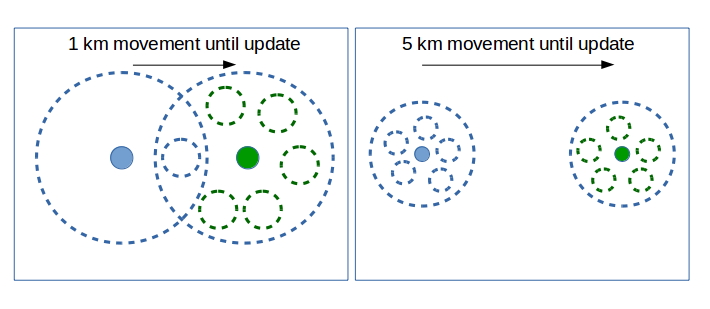
\includegraphics[width=0.9\textwidth]{images/movement_update.png}\\
	\caption{Continuous and Discontinuous location update after movement to section lacking area details  }
	\label{fig:introduction_movement_update}
\end{figure}
\FloatBarrier

\section{Location data characteristics for Berlin area}

\subsection{General overview}

Movement triggered data from mobile devices are spanned across the Germany as shown on \autoref{fig:introduction_ger_points}. 
\\
\begin{figure}[!ht]
	\centering
	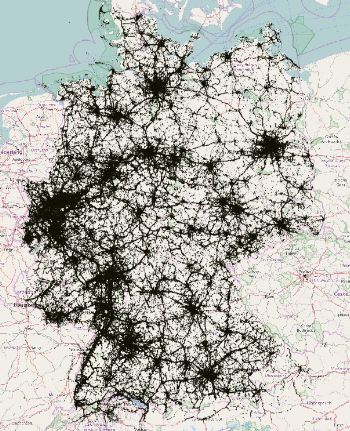
\includegraphics[width=0.3\textwidth]{images/points_germany.png}\\
	\caption{Visualisation of data points location in the geographical map of Germany}
	\label{fig:introduction_ger_points}
\end{figure}
\\
It points out, that most of the detected movements from one point to another are mostly gathered on the highways and inside the cities. 
\\
\begin{figure}[!ht]
	\centering
	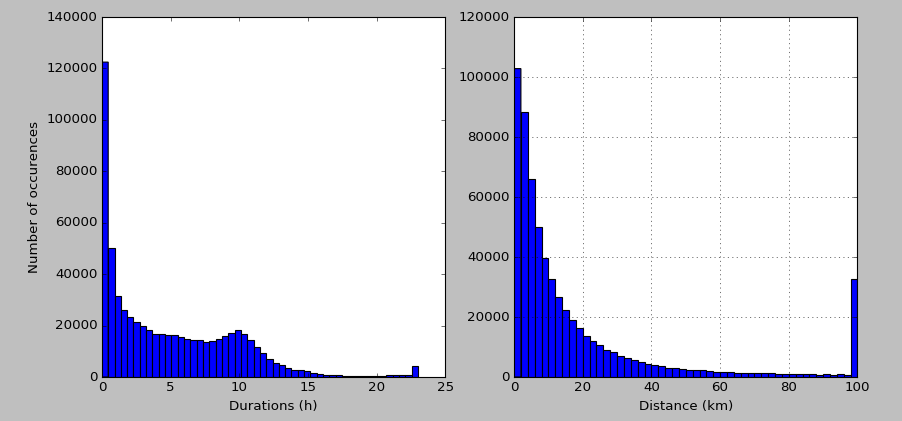
\includegraphics[width=0.9\textwidth]{images/germany_stats.png}\\
	\caption{Histograms of durations and distances between consecutive points under and cumulatively over 100 km for the area of Germany}
	\label{fig:introduction_ger_stats}
\end{figure}
\\
The given data batch has been gathered in the interval of 24h starting from 3am in the morning German time. It consists of over 675000 data points, belonging to 47300 unique mobile devices. \autoref{fig:introduction_ger_stats} shows, that for unique mobile devices, the durations between consecutive points in time are most frequent within 30 minutes and most of the data is in the interval 1-10h. Regarding distances, consecutive points are most frequent below 2 km and most data is in the interval 0-10km. Big chunk of distances is also over 100km.     
\\
\begin{figure}[!ht]
	\centering
	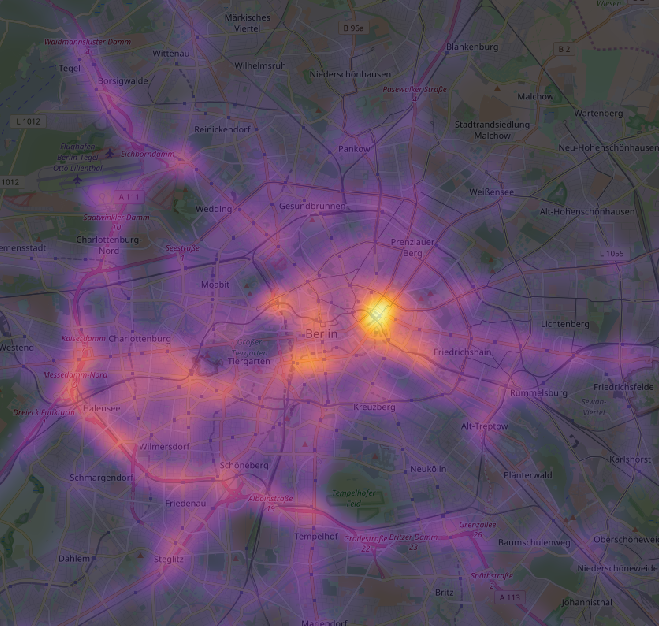
\includegraphics[width=0.9\textwidth]{images/points_berlin_heatmap.png}\\
	\caption{Heatmap of data point densities within the area of Berlin}
	\label{fig:introduction_ber_heat}
\end{figure}
\\
\autoref{fig:introduction_ber_heat} shows the heatmap of data points for Berlin area. We can see that most of the movements detected are on major train/tram/metro stations, highways and major living areas. 

\subsection{Data analysis}
\label{cha:introduction_dataanaly}

Statistics performed using tool written in Python (https://github.com/mrow4a/macroscopic-movements-algorithm-prototypes) shows, that for users at least once visiting Berlin, had in average 17 points gathered because of their movements in the period of 24h, harmonic mean of 4 points and maximum 100 of points.

\autoref{fig:introduction_ber_stats} shows that there is significant fraction of points which timestamp or distance did not change, thus duplicated point has been recorded. 
\\
TODO: This needs to be investigated
\\
\begin{figure}[!ht]
	\centering
	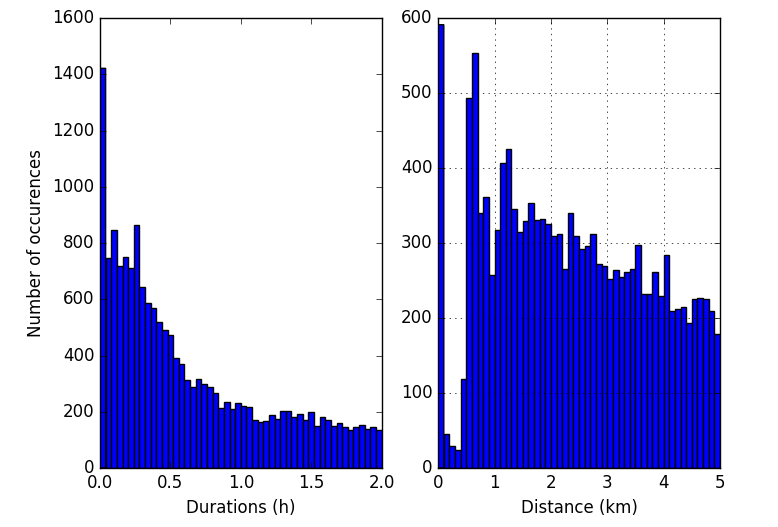
\includegraphics[width=0.6\textwidth]{images/berlin_stats_intro.png}\\
	\caption{Histograms of durations and distances between consecutive points under 5 km and under durations of 2h for the area of Berlin}
	\label{fig:introduction_ber_stats}
\end{figure}
\\\\
Furthermore, majority of durations between points is within interval of 30 minutes. For distances between points, there is significant "jump" at 500-1000m and 1100-1500m, which might mean that at these intervals, continuous points been gathered, and distances over that values might be discontinuous (ref. \autoref{fig:introduction_movement_update} ). It is due to the fact that these distance intervals are most frequent and that might suggest that this is an average "update" distance for the moving mobile devices, as described in \autoref{cha:introduction_methodo}. Less frequent values might suggest that updates were obtained with lower accuracy (e.g. by presence inside the building, metro line or simply mobile device lag in obtaining its location) and are result of discontinuity between consecutive updates.
\begin{figure}[!ht]
	\centering
	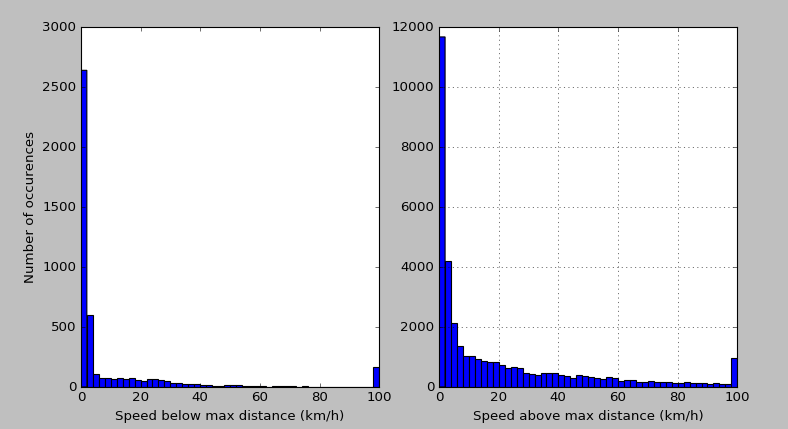
\includegraphics[width=0.6\textwidth]{images/berlin_speeds_distances.png}\\
	\caption{Histogram of speed between points with corresponding distance above or below 1.5 km}
	\label{fig:introduction_ber_sp_dis}
\end{figure}
\\
\autoref{fig:introduction_ber_sp_dis} shows that considering the registered distances within range of 1500m, the wast majority of points are between 0-2 km/h, and also significant interval at 2-6 km/h. The rest of the values is sparse distributed in interval 6-100+ km/h. In case of registered point above range of 1500m, we observe that indeed most frequent occurrence is at interval of 0-4 km/h, however most are sparse distributed above 4 km/h, with most points being in interval of 4-20 km/h. 
\FloatBarrier

\section{Approaches to stop detection for localization services}
\label{cha:introduction_appr_stopdet}

Here we should explain different approaches

\subsection{Stop Detection analyzing repetitive appearance at location}

\subsection{Stop Detection based on continuous localization}

\subsection{Stop Detection based on mobility index}
\label{cha:introduction_mob_index_sect}

In the paper \cite{MobilityIndexGIS}, movement of mobile devices between cells (handovers) is considered. To detect the periods of slow movements of stops at the specific location, parameter called Mobility Index is considered. 
\begin{figure}[!ht]
	\centering
	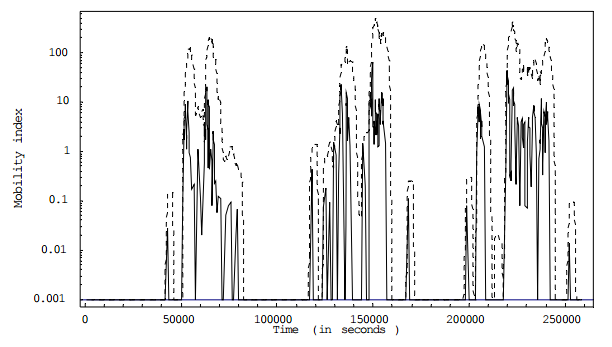
\includegraphics[width=0.5\textwidth]{images/intro_mobility_index.png}\\
	\caption{Mobility Index. Source: \cite{MobilityIndexGIS}}
	\label{fig:introduction_mob_index}
\end{figure}
\\
In a populated area, with many GSM cells, the mobile
terminal can change from one cell to another within
seconds or after several minutes. Given a set of consecutive records, the mobility of a user can be estimated by calculating the Mobility Index over a pre-defined time period (sliding window). The Mobility Index is the sum of the distance between each record and the previous ones, where the distance is the inverse of the time spent on each cell. If the value of MI is below certain threshold, it is assumed that the object stopped or moved slowly. 
\\\\
In the publication, sliding window of 10 minutes and a mobility index threshold value of 6 has been used for certain area. The obtained results were in agreement with actual movements during more than 90\% of the time. 
\\\\
High mobility index tells that user have been moving from checkpoint to checkpoint within very small time distance. Rapid drop in mobility index represents very long duration at the last point, and slight decrease in mobility index means that user changed position, but within longer duration.
%TODO \chapter{Related Work}
\label{cha:relatedwork}

\section{Human Mobility within the city}
\label{cha:introduction_hummob}

According to research \cite{HumanMobility1}\cite{HumanMobility2}\cite{HumanMobility3}, the average walking speed in the city for man aged 40 is 1.4 m/s (5 km/h), and slowest one is for elderly (with walking impairment) below 1 m/s (3.6 km/h). 

TODO: elaborate a bit more

\section{Approaches to stop detection for localization services}
\label{cha:introduction_appr_stopdet}

\subsection{Stop Detection analyzing repetitive appearance at location}

\subsection{Stop Detection based on continuous localization}

\subsection{Stop Detection based on mobility index}
\label{cha:introduction_mob_index_sect}

In the paper \cite{MobilityIndexGIS}, movement of mobile devices between cells (handovers) is considered. To detect the periods of slow movements of stops at the specific location, parameter called Mobility Index is considered. 
\begin{figure}[!ht]
	\centering
	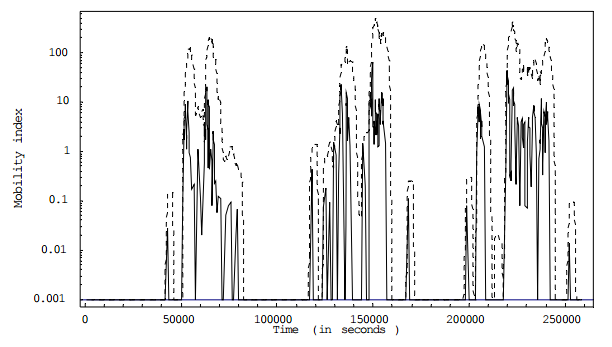
\includegraphics[width=0.5\textwidth]{images/intro_mobility_index.png}\\
	\caption{Mobility Index. Source: \cite{MobilityIndexGIS}}
	\label{fig:introduction_mob_index}
\end{figure}
\\
In a populated area, with many GSM cells, the mobile
terminal can change from one cell to another within
seconds or after several minutes. Given a set of consecutive records, the mobility of a user can be estimated by calculating the Mobility Index over a pre-defined time period (sliding window). The Mobility Index is defined as the sum of the "distances" between each record and the previous ones, where the "distance" is the inverse of the time spent on each cell. If the value of MI is below certain threshold, it is assumed that the object stopped or moved slowly. In the publication, sliding window of 10 minutes and a mobility index threshold value of 6 has been used for certain area. The obtained results were in agreement with actual movements during more than 90\% of the time. 
\\\\
Rapid drop in mobility index represents a set of points (restricted area) in which user has been moving slowly or stopped. Slight decrease in mobility index means that user changed position from restricted area and is moving.
\chapter{Concept and Design}
\label{cha:conceptanddesign}

This section is a theoretical introduction to the modules required for macroscopic movements modeling and visualization. There are three main modules in this project which can work independently from each other:

\begin{itemize}  
\item Stop location detection
\item Clustering of detected stops 
\item City Movements Graph and Analysis
\end{itemize}

\section{Type of data available}

The data supplied to the system is based on tracking and geofencing proactive location-based
service, targeted at end users and retailing companies, as discussed in \autoref{cha:introduction_hummob}. The accuracy of user location is biased not only on accuracy of position estimation used by mobile device, but also by the technological and commercial limitations of the data acquisition strategy of geofences. This means that data is spatially sparse, coarse and its resolution depends on density of geofences.
\\\\
Thus, recorded data points are associated with unique user id, timestamp, latitute and longitude of the position at which user have been found to move from one area to another.

\begin{figure}[!ht]
	\centering
	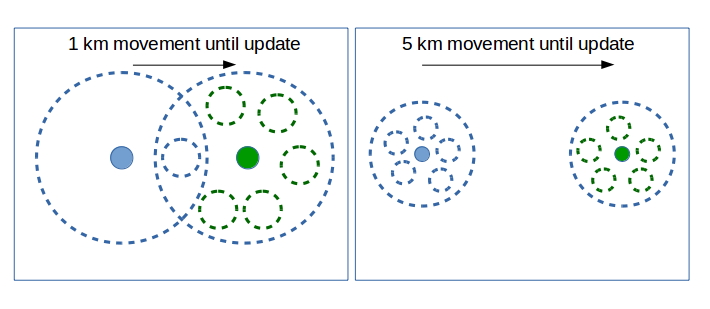
\includegraphics[width=0.9\textwidth]{images/movement_update.png}\\
	\caption{Continuous and Discontinuous location update after movement to section lacking area details }
	\label{fig:movement_update}
\end{figure}
\FloatBarrier

Because of the characteristics of GPS and other positioning methods, in so called urban street canyons and the like, signal loss with re–acquisition times of 45 seconds to five minutes can be observed \cite{StopDet1}. This could lead to discontinuous recording of the location - \autoref{fig:movement_update}.

Another aspect to consider is the fact that because of commercial application of the available data might be targeted to a specific user group, the macroscopic movements analysis might not be representative for the population in general (for example, position data  collected from a running application would probably generate different points the one for finding restaurants).

\section{Stop location detection}

In the context of macroscopic movements of people, stop detection is required to identify, based on supplied data source, whether the person under observation has stopped, at what location and how long he stayed at that location. The challenge for stop detection, in the context of proactive location-based services, is the method of data collection. Firstly, each location is recorded due to movement from one area to another. This means, that person might have stopped somewhere in between these points, and stop detection should be able to identify both location and duration of stay. Furthermore, if a user enters an urban canyon, building or move underground, the signal might need to be re-obtained after a movement to new area. This loss of signal can take some time, where points possibly can be spanned over mid-range/long distances. On the other hand, points received over a short distance might mean that a person has been already been moving with a good signal reception .

\subsection{Mobility index based approach}
\label{cha:stopdet_mi}

We decided to reuse the concept of mobility index, having artificially created areas in the city. In this case, the location point is recorded whenever moving into a new geographical area and requesting an update.
\\\\
In a populated area, the user can move from one area to another, and the movement can take from seconds to several minutes. Thus, if within a certain
period of time (called mobility index time window) the user stays in the same area or changes the areas with small pace (mobility index is below certain threshold) it can be assumed that the user is immobile or approaching stop location and having a stay somewhere within that time window (restricted area). 
\\\\
There are two approaches to calculate mobility index - having equally spaced windows in time, or sliding window.

\begin{figure}
	\centering
	\begin{minipage}{.45\textwidth}
		\centering
		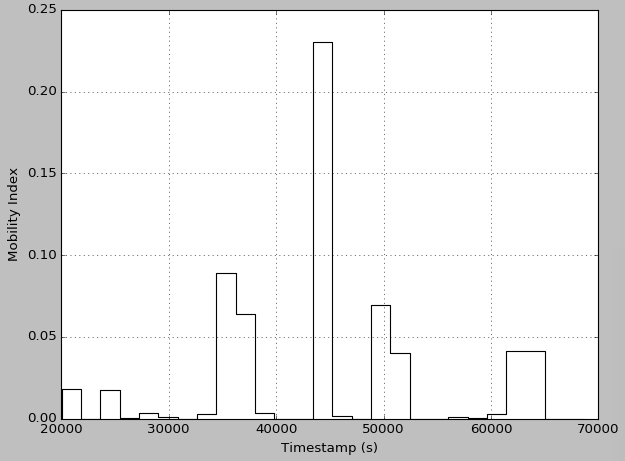
\includegraphics[width=.9\linewidth]{images/mob_calc1.png}
	\end{minipage}%
	\begin{minipage}{.45\textwidth}
		\centering
		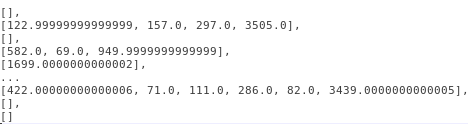
\includegraphics[width=.9\linewidth]{images/mob_calc2.png}
	\end{minipage}
	\captionof{figure}{Mobility Index calculation using equally spaced windows in time (left) and using sliding window over time (right). Time Window of 30 minutes using the same data set for one unique user}
	\label{fig:mob_calc}
\end{figure}

\FloatBarrier

In the first approach, for a single user, minimum and maximum timestamp of sorted sequence is found. The function is creating equally spaced bins of that value within the maximum and minimum timestamps. Each point is visited and assigned to the proper timestamp-bin according to its timestamp and duration to the previous point. 
The disadvantage of this approach is that points and their duration are randomly placed in bins, which could lead to representing mobility of fixed window, instead of mobility history for points.  
\\\\
In the second approach each point of a user is being visited and temporarily marked as "current position". For each current position, all points which are distant in time by the mobility index window in the past are assigned to the sliding window. The advantage of this approach is that it precisely represents the mobility history in the past duration window.

\subsection{Human Behavior based approach}
\label{cha:stopdet_bh}

This section describes the approach and conditions for movement between two points that has to be satisfied in order for the point to be a considered a stay. 
\\\\
The \autoref{cha:introduction_hummob} discusses, that in average, a walking human is traveling with the speed of over 3km/h up to 5km/h. However for movement over long distances, a user will most likely use a city or private transport, thus her speed might vary drastically in that time/distance period.
\\\\
This approach states, that if movement between two points has been recorded within short distance, and movement of speed is below a certain threshold, it might mean that user has stopped or has been moving very slowly within a restricted area. This is called a \textbf{possible stop} for that location between these points. 
\\\\
For movements between points over mid/long distances recorded, a user might have stopped at the first location, moved with different speeds between points and then continued moving (proactive localization is used). As an example, movement over 6km might require up to 10 minutes with transportation. If the user stopped at previous location for 20 minutes, the total movement between point took 30 minutes, which in average is about 12 km/h. Universal speed threshold is not able to detect stops in these kind of examples, since travels over higher speeds with stop at previous location would result in relatively high average speed. 

\section{Clustering of stops}

After our stop detection algorithm has detected the proper stops we need to analyze them. Our goal is to retrieve the overall movement patterns of a population within a certain area, which means we are interested in \textbf{macroscopic} movements and not microscopic (individual) movement. If we would consider every individual our analysis algorithms would get fed with a lot of noise (outliers) which would make data mining and prediction difficult and inaccurate. Meaning, \textit{Macroscopic Movements} are not interesting in tracking individuals but rather seeing the big picture.

 Once the clustering algorithm has been applied and we have the overall picture, we can see which stops are most popular, where people are moving from them, and how long they stay at a certain location. One could then perform some interesting graph analysis on these locations, answering questions such as "what is the probability that a person moves from point \textit{A} to \textit{B}?", or "what is the average stop time at location \textit{A}?". 
 
 To achieve these clusters, which represents our interesting stop locations, we need to apply some clustering algorithm. DBSCAN, described in \autoref{cha:relatedwork}, was our approach of achieving these clusters.  

\FloatBarrier
\section{City movements graph}
\label{cha:movementsGraph}
This section introduces the concepts and terms related to graph analysis used in this project. Our target is to identify popular locations and routes in a city and determine movement patterns of people. The stop points identified by the stop algorithm correspond to actual physical locations in the city with individual latitude and longitude values. These stop points are clustered to identify places of interest in the city. A collection of such stop clusters can be used to chart the movement patterns of the residents.

\subsection{Basic concepts}\label{cha:basicConceptsGraph}The first step of creating a user movement graph is to create vertices and edges.It is important to outline how the vertices and edges have been selected for creating the city graph. \linebreak
\textbf{Vertices:}Clusters generated by the DBSCAN algorithm are considered as vertices. \linebreak
\textbf{Edges:}For our analysis we are using an edge to represent the trajectory of movement. A trajectory or simple edge is created by joining successive points from individual user movement data.
\linebreak
\textbf{Graph:}The edge set has been used to create a simple directed graph. Direction of movement is considered from the start point going towards the end point or next point in sequence.

An important aspect about our data is that it has been captured over a period of 24 hours. In other words, our user data does not vary over days of a week. In case of such temporal variation of data, day of the week has to be considered while creating the edges.

\subsection{Graphical representation and analysis}
\label{cha:graph1}
 We are using various characteristics of a graph like in- and out-degrees, strongly connected components, betweenness and PageRank \cite{page1999pagerank} for our analysis. We are also using the concept of Origin-Destination Matrix and using the trip counts for modeling the network graph. 
 
 As mentioned in \autoref{cha:graphrelatedworks} , OD matrix is widely used in mobility data analysis and can be used to predict movement patters, important routes etc. From incidence relation between an edge and a vertex, we can calculate degrees(in and out degrees), and can identify hotspots in a city. For example: the central train station or airport of a city will have a high in and out-degree, due to high number of people traveling to and from that place.

 We will be analyzing our directed graph for strongly connected components, betweenness and PageRank. Strongly connected component can give us the areas of the city that are highly interconnected. This connection or route can be roads or transportation networks. For our mobility data, PageRank can provide us with a set of vertices that are most influential or highly accessed. Similarly, betweenness can provide us with nodes that are part of many shortest routes and hence influence the routing decisions by users. For a city, these vertices can correspond to transportation hubs, central business or administrative districts, junction or crossover points.

\FloatBarrier
\FloatBarrier
\chapter{Implementation}
\label{cha:implementation}

This chapter provides the reader understanding of the project organisation, architecture and algorithms used.

\begin{figure}[!ht]
	\centering
	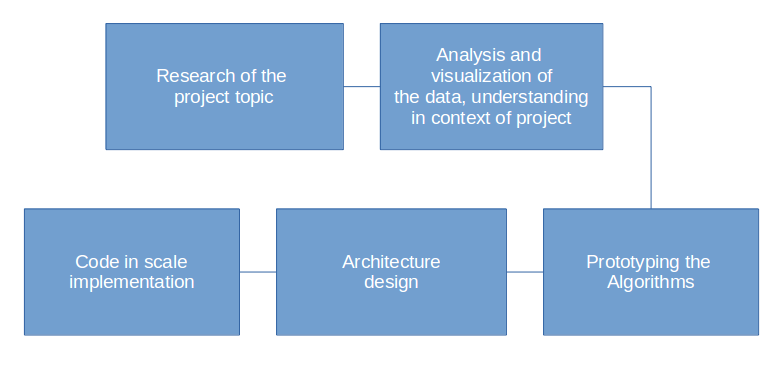
\includegraphics[width=0.6\textwidth]{images/workflow.png}\\
	\caption{ Project workflow }
	\label{fig:workflow}
\end{figure}
\FloatBarrier

At first, we researched the topic of LBS, stop detection, clustering and graph theory. Second step was to understand the data, start prototyping the algorithm for stop detection and visualize. Third step was to build four independent components using Apache Spark API and Scala - stop detection algorithm, clustering, graph analysis and web server. Fourth step was to build a scalable architecture and mock additional 3rdparty components (Minio S3 and Apache Spark containers).

\section{Scripts for data analysis in python and QGIS}

To understand the data we have used a set of tools in python \cite{pythonQgis}. These enabled us to quickly understand the data in general (nubmer of users, avarage number of points, average duration, distance, speed etc) and per user (plotting distances and speeds between points in time). We also extensively used a tool called QGIS in order to visualize data on the map. 

\section{Architecture - batch processing in Apache Spark}

The architecture of the project follows an elegant microservice concept, using independent deployable components.
The project primarily consists of three independent components; S3 storage (a protocol for data storage, in this case open source \textit{Minio} in Docker container), Apache Spark cluster (distributed compute engine over nodes), and a web server with spark jobs and spark-submit. See figure \autoref{fig:architect}.

\begin{figure}[!ht]
	\centering
	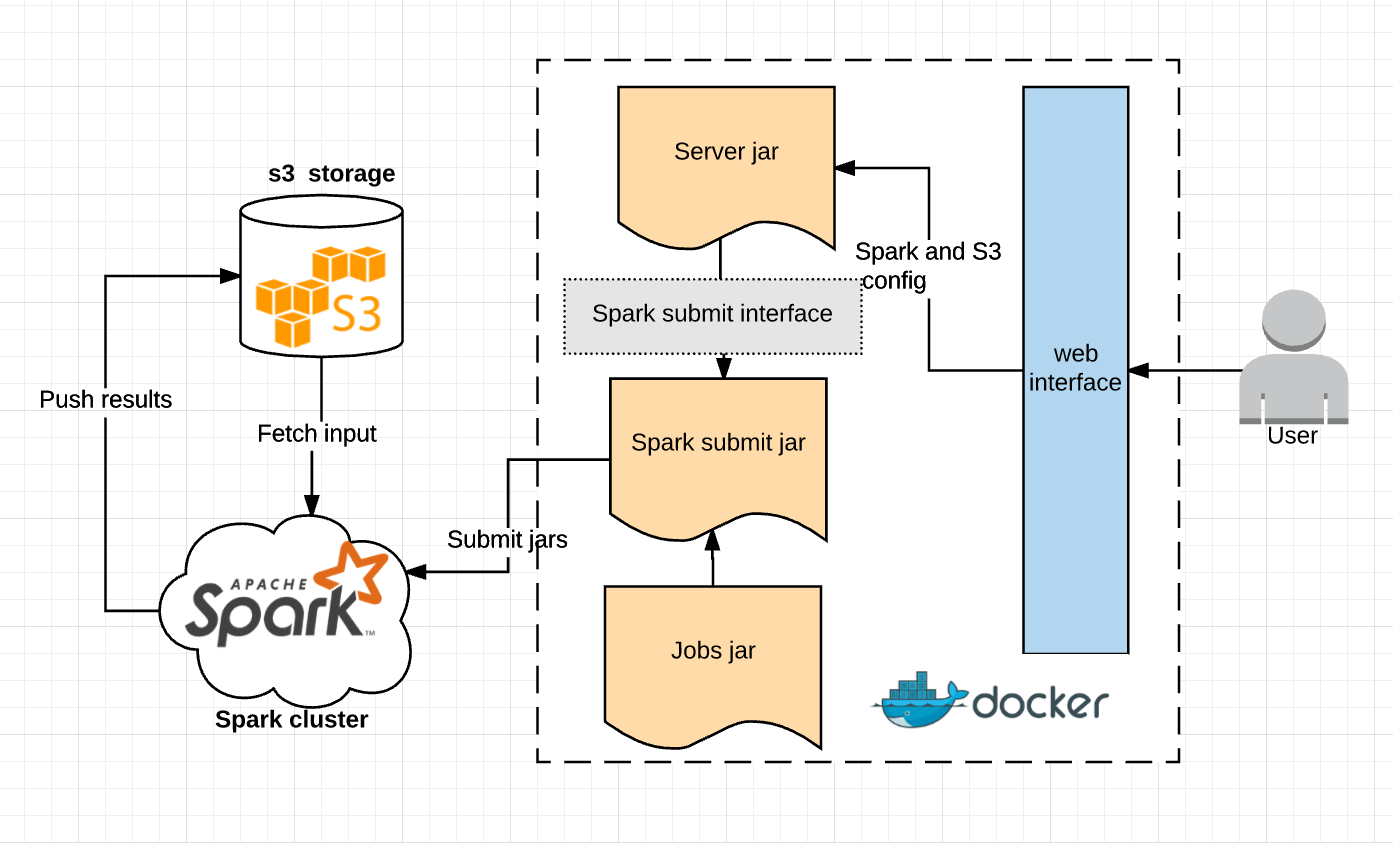
\includegraphics[width=0.8\textwidth]{images/architect.png}\\
	\caption{ Architecture of implemented project, using s3, spark, and docker}
	\label{fig:architect}
\end{figure}
\FloatBarrier

The stop detection jobs are bundled in jars and submitted through the \textbf{Spark submit interface} to the \textbf{Apache Spark cluster}. They will there be load balanced over the slaves by the Spark master which fetches the input file from the \textbf{s3 storage}. This storage can be local or deployed on a shared cloud service. After the computation is finished the master can push data back into the \textbf{s3 storage}.

To easily deploy the application and make it environmental agnostic we bundled everything into the container platform Docker. 

Let us describe a basic scenario:

\begin{enumerate}
  \item 
User starts the docker containers which will start spark cluster and s3 storage.
  \item 
User uploads the input file on to the S3 storage.
  \item 
User runs docker container containing the project code (macromovements jobs jar, spark submit jar and web server jar)
  \item 
User accesses the web interface, provide configuration such as the url of the input file (in S3) and the url where the Spark master resides.  
  \item 
User runs the stop detection job from the web interface by pressing the "setup" and "run" buttons. Output will be displayed using Leaflet Javascript library on the map
\end{enumerate}

\section{Determining stop location}
\label{cha:stopdet_impl}

This section discusses implementation details of the algorithm used to identify stops. \autoref{fig:stop_algo} shows block diagram of stop detection algorithm. The input to the algorithm is list of vectors containing at its first 5 elements day of the week, time of day, user id, latitude and longitude of the recorded location. 

\begin{figure}[!ht]
	\centering
	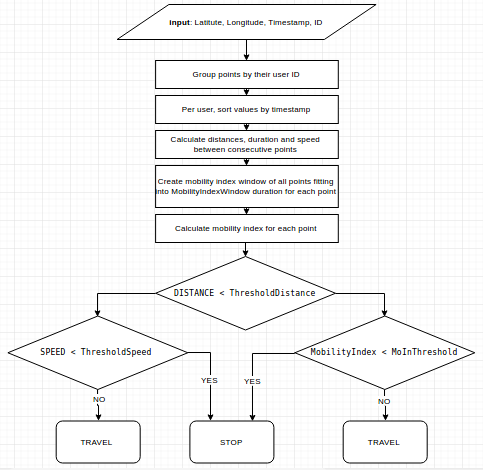
\includegraphics[width=0.95\textwidth]{images/stop_algo.png}
	\caption{ Stop detection algorithm for proactive localization services. }
	\label{fig:stop_algo}
\end{figure} 

\FloatBarrier

The first phase of stop detection algorithm is to group points according to user id. As algorithm is implemented in Spark, each user is processed in parallel. Per user, values are sorted according to their timestamp. Distance, speed and duration is calculated for each consecutive pair of points. Values are being filtered for anomalies in the next step. Mobility Index for each point is calculated, as discussed in \autoref{cha:stopdet_mi}. Further, decision based on thresholds is made whether the point is stop or not. 


\section{Clustering}

%TODO descib in related work
 The implementations of clustering were primarily done by using open source implementations and extending it to our needs. For clustering we used the algorithm DBSCAN. 
 
We wanted a scalable implementation of DBSCAN that could handle large data sets, preferable in parallel. We decided to use Apache Spark, a scalable engine for large-scale data processing \cite{spark}. For this we used an implementation by Irving Cordova, explained in Related work, \autoref{cha:relatedwork}. 

Along as using this implementation we extended it with an area version, which divided the data set into predefined boxes. Each box were assign different parameters (discussed in Evaluation, \autoref{cha:evaluation} and ran in parallel. After each box was finished the results were merged and written to a file along with important output (such as latitude, longitude, user id, cluster id).

Other versions of DBSCAN were also implemented that ran the jobs in batches and stored it in different files, used for evaluating the results and plotting them in the graph visualization tool QGIS.


\section{Analyzing the user movement graph}
We have used GraphX and Python for creating and analyzing the user movement graph. GraphX was used for creating the data sets and the graph. Before creating the graph, we filtered the data and structured it in a suitable format. 

Filtering was essential at this step as the clustering algorithm identified many stop points as outliers with cluster id=0. We filtered out these outliers from the main data set. With the filtered data, our task was to determine the vertex and edge sets. We used trip count values for each source destination pair as the edge weight. Next task was to create the graph.
 
GraphX provides built-in functions to extract many different properties of a graph. We used GraphX for the indegrees, outdegrees and PageRank values and also NetworkX library of Python to obtain the strongly connected components and betweenness values of our graph. We plotted the results using Python so that we could form a better understanding of the data. It also helped us determine thresholds while calculating top indegree, outdegree, pagerank and betweenness values. We also used the tool QGIS to visualize the property values with respect to physical locations in cities.

\section{User Interface}
To bundle our three parts; stop detection, clustering of detected stop, and graph analysis we developed a web based user interface where job files could be submitted to a running Spark cluster from a specified Amazon S3 storage. The UI was build upon leaflet\cite{leaflet}, a interactive map library for JavaScript, and featured functionality for running the jobs, displaying  the clusters and visualizing graph information such as connected component with out and in degree. To minimize executing time we implemented functionality for displaying previously ran job, instead of re executing jobs it could now display previously ran jobs. When a stop is clicked statistics about the stop appears and lines are drawn on the map according to the out and in degrees (connected travellers to/from this stop to another captured one) See figure \autoref{fig:ui_berlin}

The current UI provides following features:
\begin{itemize}
  \item Interactive world \textbf{map} for zooming and panning
  \item \textbf{S3 input file for ETL}: S3 bucket and file name of the input job (currently csv file)  
  \item \textbf{Spark master address}: URL of the spark master that should process the job
  \item \textbf{S3 storage URL}: The URL of the running S3 instance (could be local or public)
  \item \textbf{Test}: Test if job is OK and we can connect to Spark and S3
  \item \textbf{Run}: Run the job and display it on map (in case of a result file, just display the result)
  \item \textbf{Export to CSV}: Download the result output as a csv file for further use, such as not having to re-run the job again. 
  \item \textbf{Statistics about stop}: Panel displaying information  graph information about the clicked cluster, such as id, size, in/out degrees, PageRank etc. 
\end{itemize}

\begin{figure}[!ht]
	\centering
	\includegraphics[width=1\textwidth]{images/ui_berlin.png}\\
	\caption{ Screenshot of the user interface }
	\label{fig:ui_berlin}
\end{figure}
\FloatBarrier

\newcolumntype{L}{>{\centering\arraybackslash}m{4.5cm}}

\chapter{Evaluation}
\label{cha:evaluation}
 
\section{Location data characteristics for Berlin area}

\subsection{General overview}

Movement triggered data from mobile devices are spanned across the Germany as shown on \autoref{fig:ger_points}. 
\begin{figure}[!ht]
	\centering
	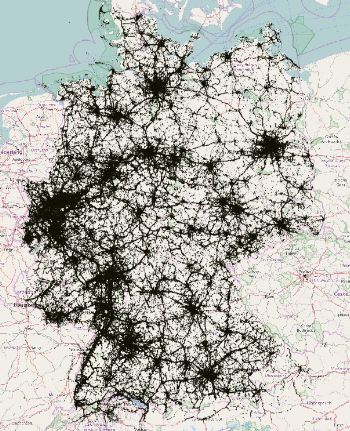
\includegraphics[width=0.3\textwidth]{images/points_germany.png}\\
	\caption{Visualisation of data points location in the geographical map of Germany}
	\label{fig:ger_points}
\end{figure}
\FloatBarrier
It points out, that most of the detected movements from one point to another are mostly gathered on the highways and inside the cities. 
\\
\begin{figure}[!ht]
	\centering
	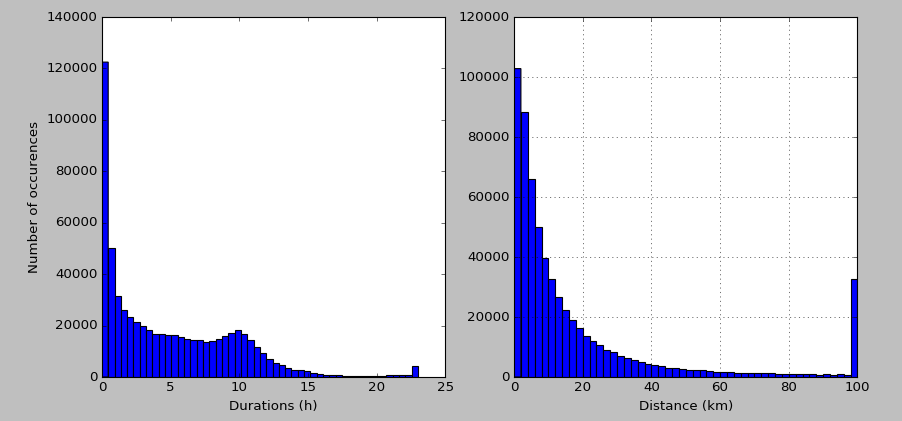
\includegraphics[width=0.9\textwidth]{images/germany_stats.png}\\
	\caption{Histograms of durations and distances between consecutive points under and cumulatively over 100 km for the area of Germany}
	\label{fig:ger_stats}
\end{figure}
\FloatBarrier
The given data batch has been gathered in the interval of 24h starting from 3am in the morning German time. It consists of over 675000 data points, belonging to 47300 unique mobile devices. \autoref{fig:ger_stats} shows, that for unique mobile devices, the durations between consecutive points in time are most frequent within 30 minutes and most of the data is in the interval 1-10h. Regarding distances, consecutive points are most frequent below 2 km and most data is in the interval 0-10km. Big chunk of distances is also over 100km.     
\\
\begin{figure}[!ht]
	\centering
	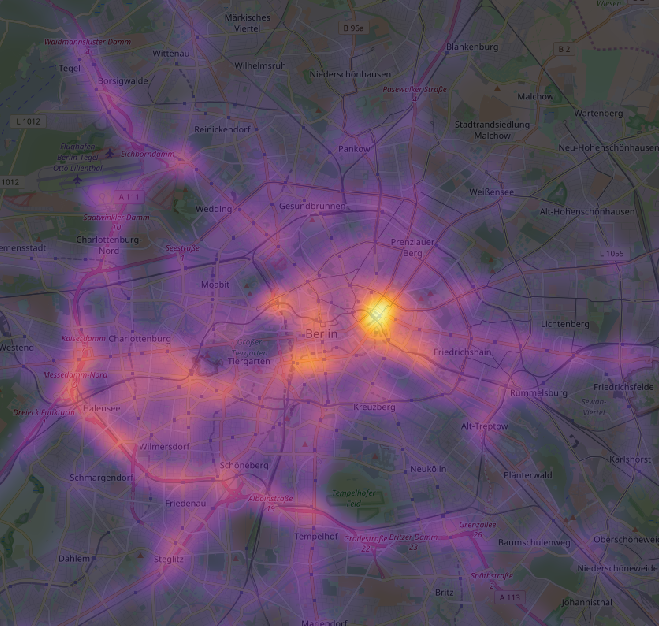
\includegraphics[width=0.9\textwidth]{images/points_berlin_heatmap.png}\\
	\caption{Heatmap of data point densities within the area of Berlin}
	\label{fig:ber_heat}
\end{figure}
\FloatBarrier
\autoref{fig:ber_heat} shows the heatmap of data points for Berlin area. We can see that most of the movements detected are on major train/tram/metro stations, highways and major living areas. 

\subsection{Data analysis}
\label{cha:dataanaly}

Statistics performed using tool written in Python (https://github.com/mrow4a/macroscopic-movements-algorithm-prototypes) shows, that for users at least once visiting Berlin, had in average 17 points gathered because of their movements in the period of 24h, harmonic mean of 4 points and maximum 100 of points.
\\
\begin{figure}[!ht]
	\centering
	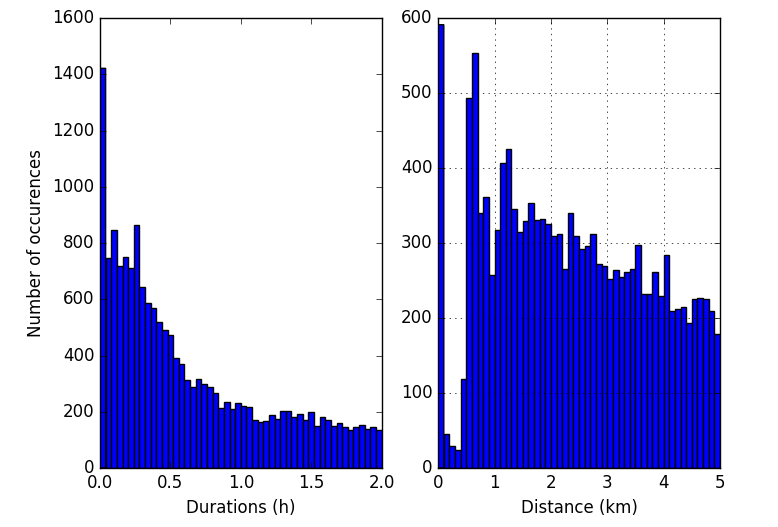
\includegraphics[width=0.6\textwidth]{images/berlin_stats_intro.png}\\
	\caption{Histograms of durations and distances between consecutive points under 5 km and under durations of 2h for the area of Berlin}
	\label{fig:ber_stats}
\end{figure}
\FloatBarrier
Furthermore, majority of durations between points is within interval of 30 minutes. For distances between points, there is significant "jump" at 500-1000m and 1100-1500m, which might mean that at these intervals, continuous points been gathered, and distances over that values might be discontinuous (ref. \autoref{fig:movement_update} ). It is due to the fact that these distance intervals are most frequent and that might suggest that this is an average "update" distance for the moving mobile devices, as described in \autoref{cha:introduction_methodo}. Less frequent values might suggest that updates were obtained with lower accuracy (e.g. by presence inside the building, metro line or simply mobile device lag in obtaining its location) and are result of discontinuity between consecutive updates.
\begin{figure}[!ht]
	\centering
	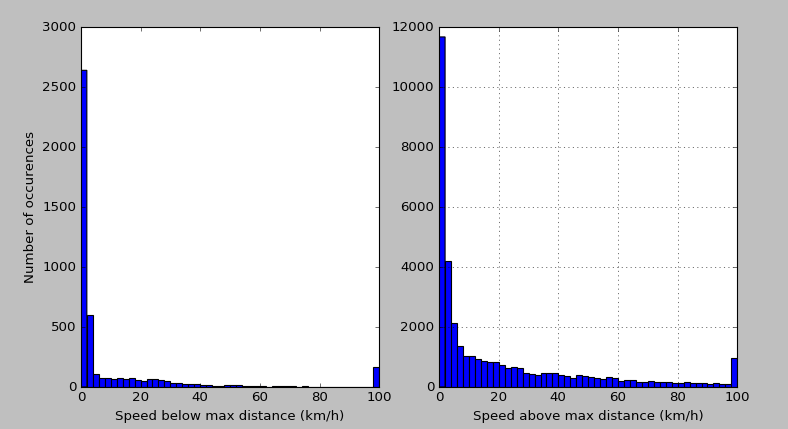
\includegraphics[width=0.6\textwidth]{images/berlin_speeds_distances.png}\\
	\caption{Histogram of speed between points with corresponding distance above or below 1.5 km}
	\label{fig:ber_sp_dis}
\end{figure}
\FloatBarrier
\autoref{fig:ber_sp_dis} shows that considering the registered distances within range of 1500m, the wast majority of points are between 0-2 km/h, and also significant interval at 2-6 km/h. The rest of the values is sparse distributed in interval 6-100+ km/h. In case of registered point above range of 1500m, we observe that indeed most frequent occurrence is at interval of 0-4 km/h, however most are sparse distributed above 4 km/h, with most points being in interval of 4-20 km/h. 

\section{Pre-filtering of anomalies}
\label{cha:prefilter}
\autoref{fig:ber_stats} shows that there is a fraction of points which duration or distance rapidly changed, thus resulting in very high speeds between the points. Points having speeds above 300 km/h and distances above 100km can be considered as flights, however the ones below 100km are anomalies. \autoref{fig:anom1} shows that number of flights in Germany has not been significant (around 100) compared to number of speed anomalies (over 25000).
\\\\
Furthermore, due to the methodology of obtaining points (movement triggered), there are some minimum distances and durations at which points can be collected, and values not matching stop or travel expectation according to gathered statistics, have to be filtered and considered as duplicates. 

\begin{figure}[!ht]
	\centering
	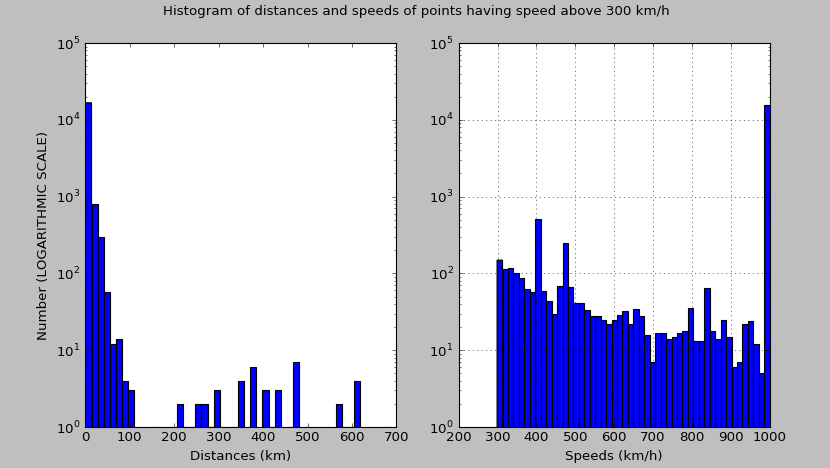
\includegraphics[width=0.6\textwidth]{images/anom1.png}\\
	\caption{ Speeds and distances histogram of points having speeds above certain threshold }
	\label{fig:anom1}
\end{figure}
\FloatBarrier

Thus, the following predicates for filtered values have been set:
\begin{description}
	\item[Jumps] Points with speed over 83 m/s [300 km/h] and at the same time distance below 100 km/h
	\item[Duplicates] Points with distance below 100m and at the same time duration below 100s
\end{description}

\section{Evaluation of stop detection algorithms}

\subsection{Mobility Index approach}

Mobility Index analysis is performed in order to detect single movements or series of movements to be classified as stop or slow movement over the restricted area. 
\\\\
By the nature of mobility index, more values in the window, higher the mobility index is. Thus, if only one value is in the window, one can apply "stop duration" threshold, however if windows contains more values, we require higher threshold to be able to fit sum of inverses of the movements. 
\\\\
As an example, having window of 20 minutes and threshold of 1/(10 minutes), if we fit into window single point with duration of 15 minutes, this value will be classified as a stop. However, if we obtain 2 values, 5 and 10 minutes respectively (1/5 + 1/10), our threshold requires to be higher in order to include slow movements in the window and classify this 2 values as stop in restricted area.

\begin{figure}[!ht]
	\centering
	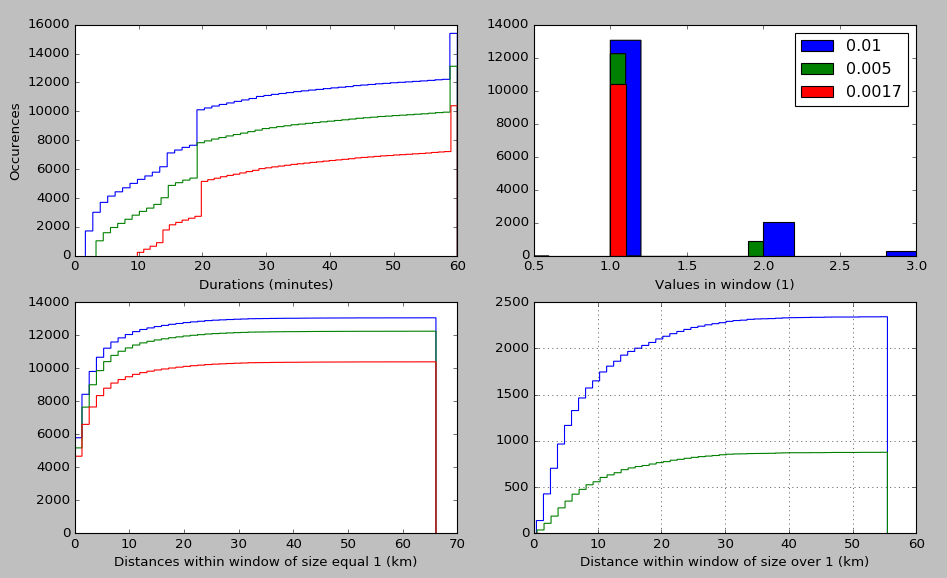
\includegraphics[width=0.95\textwidth]{images/mob_index_analy1.png}\\
	\caption{ Analysis of detected stops for varying MobilityIndexThreshold for time window of 20 minutes. Cumulative distribution of inverted mobility index (top left). Histogram of window sizes (top right). Cumulative distributions of total distances between points in the window of size 1 (bottom left) and above 1 (bottom right). }
	\label{fig:mob_index_analy1}
\end{figure}
\FloatBarrier

\autoref{fig:mob_index_analy1} shows the analysis of the stops detected using mobility index, using sliding time window approach.
\\\\
Cumulative distribution of inverted mobility index (top left) shows that for window of 20 minutes, increasing MobilityIndexThreshold from 0.0017 (1/10 minutes) to 0.01 (1/2minutes), sum of inversions of durations (MobilityIndex) for points within the window, increases total number of stops from 10000 to 15000, where the increase (5000 points) is caused by points in the range 2-10 minutes, which is expected result increasing the threshold. The rapid jump at 20 minutes is caused by the fact that at that threshold some inverted mobility indexes were result of summing window of more then one value. 
\\\\
Histogram of sizes of the window (number of points within a 20 minutes window - top right) shows, that with parameter 0.0017, all the points are contained within the windows having size of 1 point. Increasing the threshold to 0.005 (1/4 minutes), it resulted in 95 percent of points being in windows of size 1 and 5 percent in windows of size 2 (2 points in the window - restricted area of stop). Doubling the threshold to 0.01 resulted in 75 percent being in single value window, and 25 percent in over 2 points per window. 
\\\\
The graphs in the bottom of \autoref{fig:mob_index_analy1} show what are the distances covered in the windows having 1 or more points. It occurs, that in case of 1 point in the window (which means that this point is a stop), distances between points range from 0 to 60km, and this is expected. However, in case of 2 or more points per window (thus stops within a restricted area bound by points), it occurs that only small fraction of values has total distance covered less then 2km, and major fraction of points represent long distance covered. 
\\\\
The above analysis shows, that mobility index cannot be effectively used to detect group of points which might be considered as a stop and only very small fraction of windows having more points then 1 is considered as a stop within a small restricted area. The rest is spanned across bigger distances. Thus, small values of mobility index window and threshold might start detecting trips over longer distance as a stop and providing erroneous results. 
  
\begin{figure}[!ht]
	\centering
	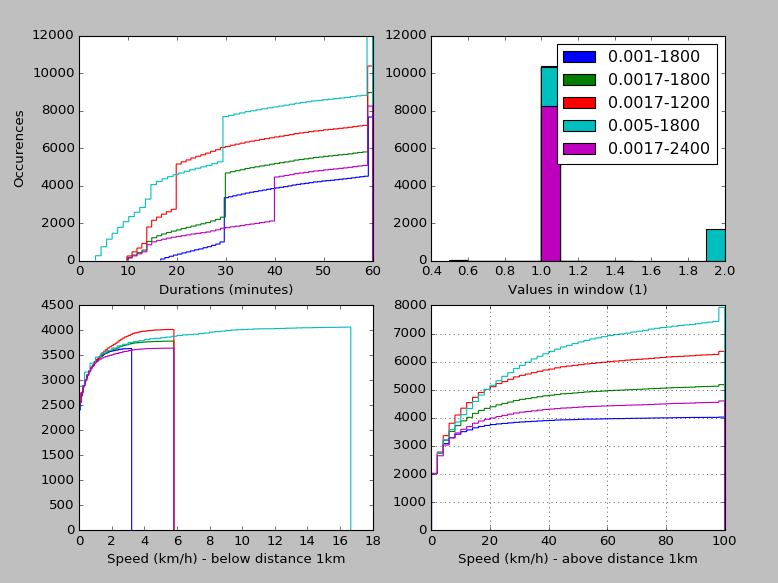
\includegraphics[width=0.95\textwidth]{images/mob_index_analy2.png}\\
	\caption{ Analysis of detected stops for varying MobilityIndexThreshold-MobilityIndexWindow(seconds), correspondingly as in the label of measurement. Cumulative distribution of duration for detected stops (top left). Histogram of window sizes (top right). Cumulative distributions of speed between point for distance below 1km (bottom left) and above 1km (bottom right). }
	\label{fig:mob_index_analy2}
\end{figure}
\FloatBarrier 
 
\autoref{fig:mob_index_analy2} shows the analysis of the stops detected using mobility index threshold, using sliding time window approach, however in this case it is used to identify mobility of a user considering only last recorded point in the window to decide if the movement can be a stop considering its past mobility.
\\\\
This approach tries to tackle the problem discussed in \autoref{cha:stopdet_bh}, where it has been said that over longer distances e.g. 2-10 km between recorded points, detection using speed is difficult since stop for a short time and movement with high speed will produce very high average speed in that time period. 
\\\\
\autoref{fig:mob_index_analy2} gives cumulative histograms considering different pair of parameters (MobilityIndexThreshold-MobilityIndexWindow) considered in producing stop locations. Cumulative distribution of duration at detected stops (top left) shows that considering the same MobilityIndexThreshold (0.0017-1200s, 0.0017-1800s, 0.0017-2400s) and increasing MobilityIndexWindow, causes less stops to be detected and higher average duration between points detected. Considering the same MobilityIndexWindow (0.001-1800s, 0.0017-1800s, 0.005-1800s) and increasing MobilityIndexThreshold, number of stops increases, and this increase is bound only to values below MobilityIndexWindow threshold. High MobilityIndexThreshold produces more stops with shorter duration of stop. 
\\\\
Cumulative distribution of speed for detected points show that algorithm with all tested parameters has been able to identify correctly stops over distance less then 1km and with very small speeds (long stay duration at the point). However, MobilityIndexThreshold or decreasing MobilityIndexWindow cause that average speed of detected points had higher speed over distances > 1km and these were not able to filter trips over long distances correctly. For thresholds 0.001-1800s, 0.0017-1800s and 0.0017-2400s higher speeds are being filtered and only longer stays are left, and the difference between performance of these parameters is a trade-off between an accuracy and number of detected stops. 
\\\\
Histogram of values in the window (top right) also confirms, that for 0.001-1800s, 0.0017-1800s and 0.0017-2400s thresholds, detected stops had window of 1 value, thus none of the windows having 2 or more values were not qualified for being a stop and thus being filtered out as high mobility trip. This behavior of algorithm allows to identify stays with simple duration threshold and at the same time filter out all multi-point trips using mobility index window. 

\subsection{Human Mobility approach for long/short distances}

Speed/Distance analysis is performed in order to detect single movements as stop or slow movement. If the average speed between the points is below the certain threshold, it is assumed to be a stop. 
 
\begin{figure}[!ht]
	\centering
	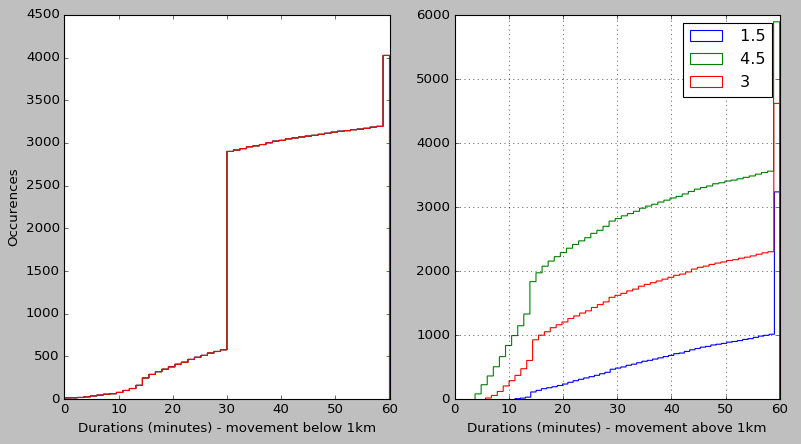
\includegraphics[width=0.95\textwidth]{images/speed_dist_analy1.png}\\
	\caption{ Speed/Distance detection with StopCertaintyMaxDistance, StopCertaintyMaxSpeed and TravelCertaintyMinSpeed thresholds. Cumulative distribution of duration for detected stops below and above distance StopCertaintyMaxDistance of 1km for different  TravelCertaintyMinSpeed thresholds. }
	\label{fig:speed_dist_analy1}
\end{figure}
\FloatBarrier 

\autoref{fig:speed_dist_analy1} shows analysis of detected stops having TravelCertaintyMinSpeed varying and StopCertaintyMaxSpeed fixed. Increasing the speed threshold for points above 1km, we observe that number of points in interval 15 to 60+ minutes stays fixed for all parameters, however increasing threshold increases number of stops detected in interval 5-15 minutes diracticaly. It means, that with these thresholds, much more movements which has very low duration over the distance are classified as a stop and identification might be erroneous to mislead long distance trip with a stop. 
\\\\
Furthermore, having TravelCertaintyMinSpeed threshold of 1.5 m/s, we can see that speed threshold correctly identifies the stops, however the number of detected stops in the movements above 1km compared to mobility index approach is low (\autoref{fig:mob_index_analy2})
\\\\
On the other hand, for distances below 1km, speed detection has not only been able to identify longer stays at location, but also a short distance, very slow movements over the area, successfully. 

\subsection{Conclusions}

\begin{table}[h!]
	\centering
	\caption{Comparison of two analyzed stop detection algorithms for proactive localization}
	\label{tab:alg_comp_table}
	\begin{tabular}{|L|L|L|}\hline
		\textbf{Case} & \textbf{Mobility Index} & \textbf{Speed/Distance} 
		\\\hline
		Slow movements over small area or distance & Possible, but adjusted parameters will cause results to be erroneous for different detections & Very good
		\\\hline
		Stays at short distance & Good, but only for longer stays & Very good  
		\\\hline
		Stays at long distance & Very good, but only in case of adjusted parameters which might be erroneous at short distances & Possible, but might be erroneous and stops maybe mislead with travel due to high speed averages in these cases
		\\\hline
	\end{tabular}
\end{table}
\FloatBarrier 

\autoref{tab:alg_comp_table} shows comparison of two approaches to stop detection. It occurs, that for short distances it is more efficient to use speed/distance algorithm to be able not only capture longer stays at short distance, but also very slow movements in the limited area. For longer distances it is preferable to use mobility index to be able distinguishing travels from stops better using mobility index, which preserves mobility history for the certain past time window. MobilityIndexWindow becomes a duration threshold at which mobility window with multiple points are being accepted, and MobilityIndexThreshold is defining which multiple points or single points cannot be classified as a stop and be a series of movements/movement. 

\section{Clustering algorithm}

In this section we will describe how we evaluated our dbscan algorithm and the choice of the \textit{epsilon} and \textit{minimum points per cluster} parameter.

\subsection{DBSCAN}

We visualised our results in QGIS, a powerful graph visualisation tool. Running the dbscan with different parameters resulted in different cluster sizes and number of clusters. We started off with the target area of Berlin. The \textit{epsilon} parameter (radius of the cluster) was chosen by looking at the graininess (accuracy) of our given data set. The accuracy between points was 110 meters, this distance is refered to as \textit{accuracy distance}.
We took Alexanderplatz in Berlin as an example cluster (a popular train stop area in Berlin). We interpret one cluster as being one stop point of interest, and for this application want Alexanderplatz to be represented as one cluster. Setting the \textit{epsilon} parameter to the \textit{accuracy distance},  110 meters, gave us good looking clusters whilst higher value of the parameter resulted in clusters being unnaturally large and distance below the \textit{accuracy distance} resulted in only single-point clusters (points are stacked at the same location). Note that the \textit{minPts}, minimum points per cluster, parameter is not taken into \textit{consideration} here (it is set arbitary and only determines the number of clusters, while we here are interested in the \textit{size} of the clusters). See figures below.

\begin{figure}[!ht]
	\centering
	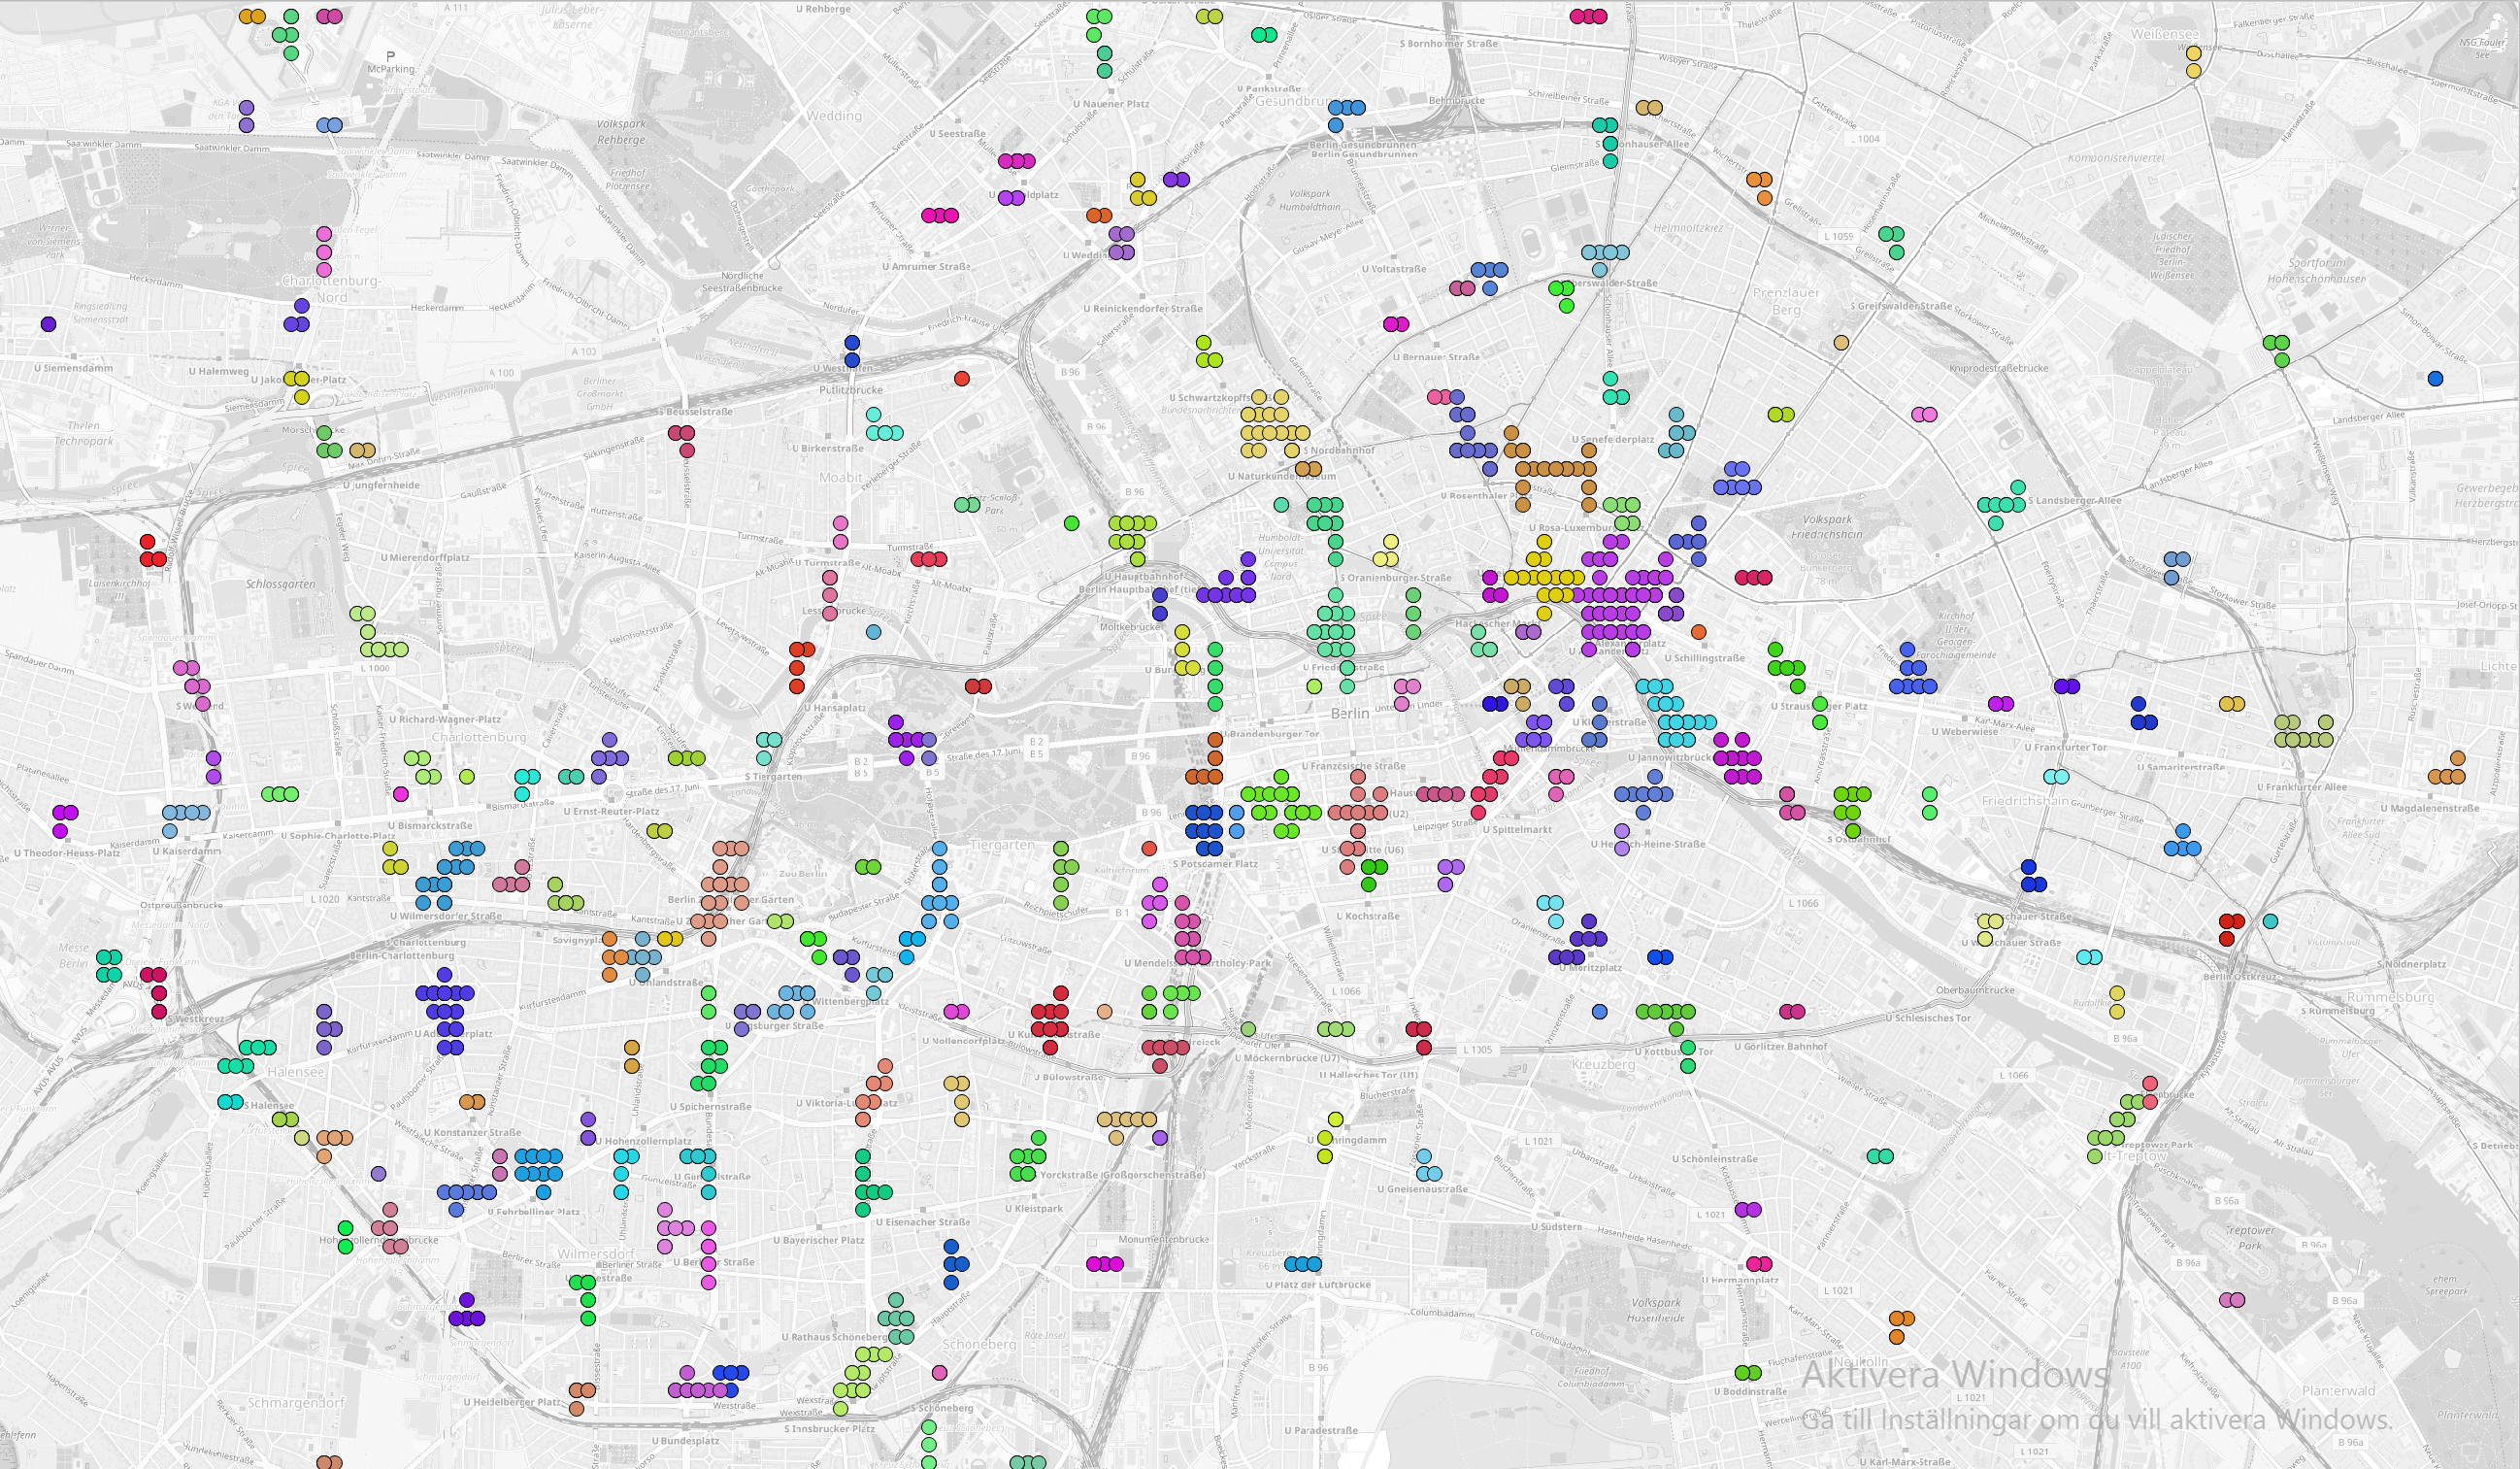
\includegraphics[width=1\textwidth]{images/0,001_5_gray.png}\\
	\caption{ Clusters with good parameters \textit{epsilon} = 110 meter, \textit{minPts} = 5. Alexanderplatz (pink) has 85 data points in it.  }
	\label{fig:0.001_5_gray}
\end{figure}

\begin{figure}[!ht]
	\centering
	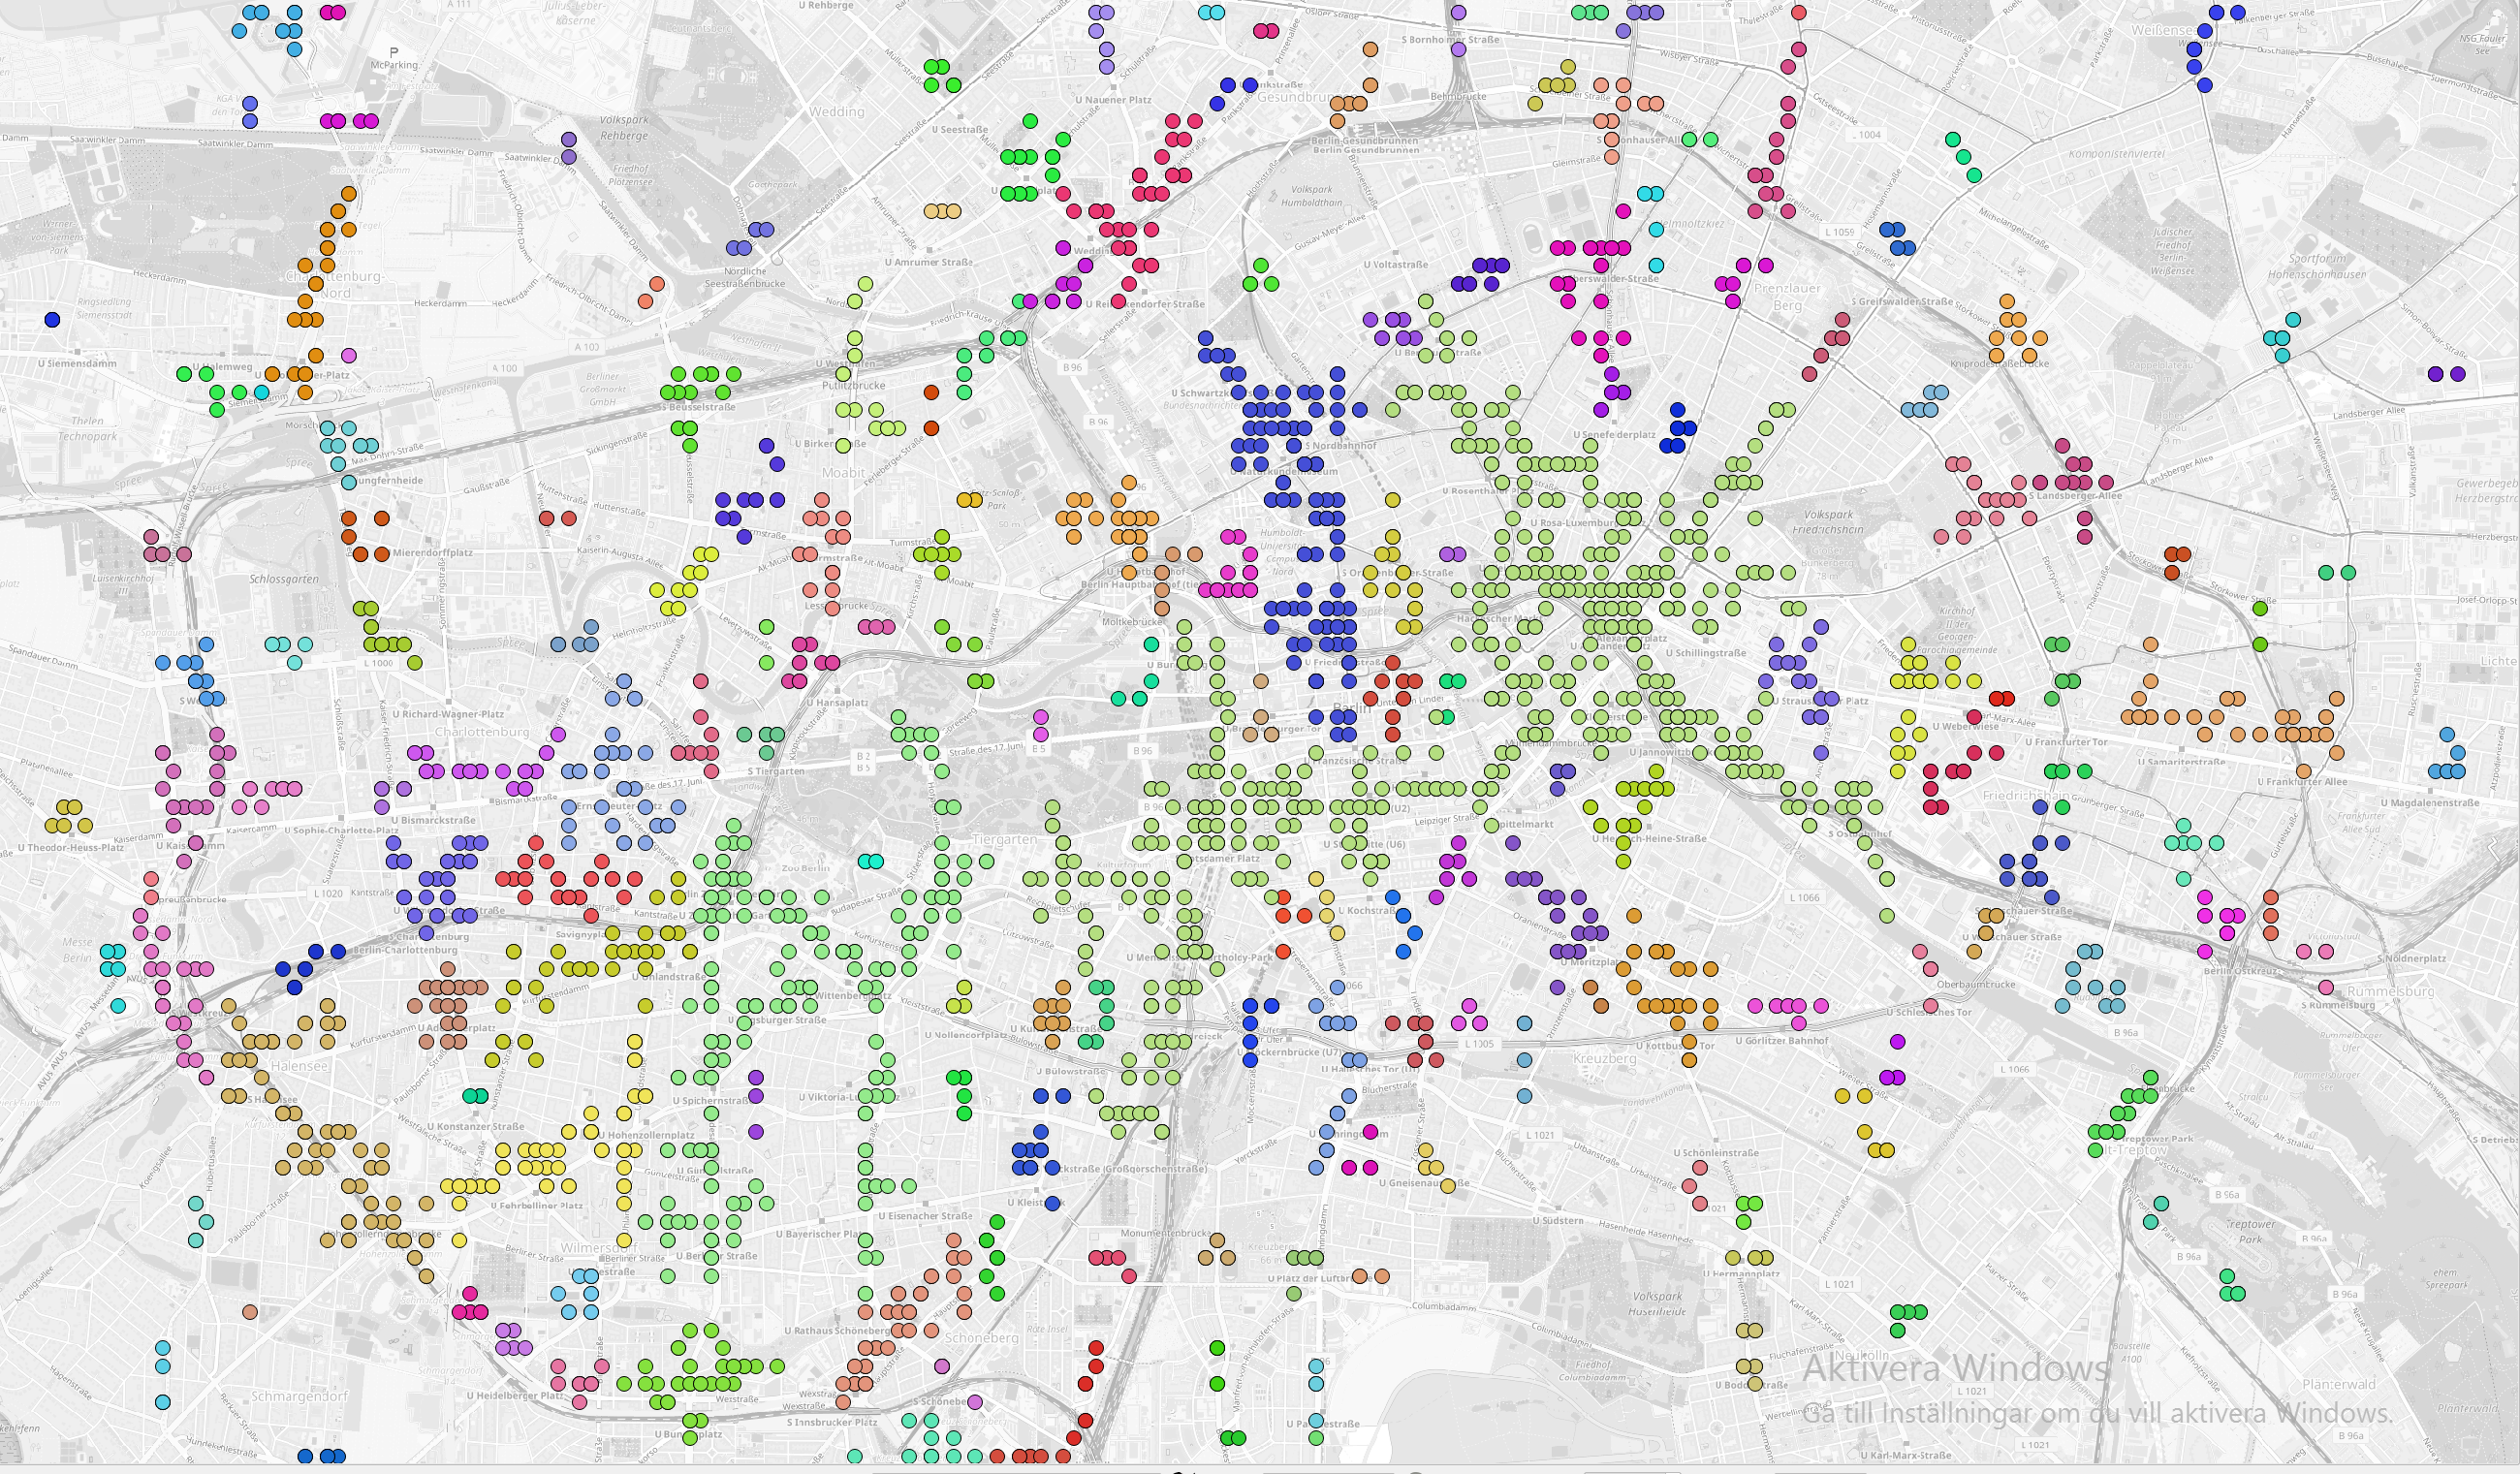
\includegraphics[width=1\textwidth]{images/0,002_5_gray.png}\\
	\caption{ Example of a clusters with bad parameters, here \textit{epsilon} = 220 meter is too large, \textit{minPts} = 5. "Alexanderplatz" (light green) has 748 data points in it and stretches over the whole centre (Mitte) of Berlin. }
	\label{fig:002_5_gray}
\end{figure}
%TODO\chapter{Conclusion}
\label{cha:conclusion}

Describe what you did here

%--------------------------------------------------------------
% TABLES, FIGURES, BIBLOGRAPHY AND APPENDICES
%--------------------------------------------------------------
\backmatter

% Lists of tables and figures
%TODO \listoftables
%TODO \listoffigures

% Bibliography
\setwidesite{}						% Set page to be wider for bibliography
\markboth{Bibliography}{Bibliography}
\label{cha:bibliography}
\printbibliography

% Use following to separate online (websites) and offline (books, papers) sources
%\printbibliography[heading=offline,filter=offline]
%\printbibliography[heading=online,filter=online]

\begin{appendices}
	\chapter{Appendix 1}
\label{appendix:add_example_1}

\begin{figure}[!ht]
	\centering
	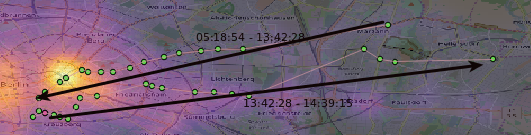
\includegraphics[width=0.6\textwidth]{images/reco_example_3a.png}\\
	\caption{ Visualization of distances, speed and mobility indexes for example from \autoref{fig:reco_ex_3b} with identified stop candidates }
	\label{fig:reco_ex_3a}
\end{figure} 
\begin{figure}[!ht]
	\centering
	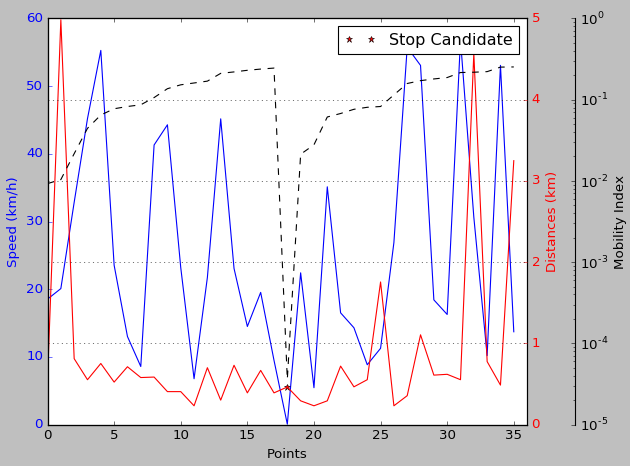
\includegraphics[width=0.6\textwidth]{images/reco_example_3b.png}\\
	\caption{ Movement example for one user in the period of 24h, with recorded locations due to the movement and annotated timestamps for detected stop candidates }
	\label{fig:reco_ex_3b}
\end{figure}
	\chapter{Appendix 2}
\label{appendix:add_example_2}

\begin{figure}[!ht]
	\centering
	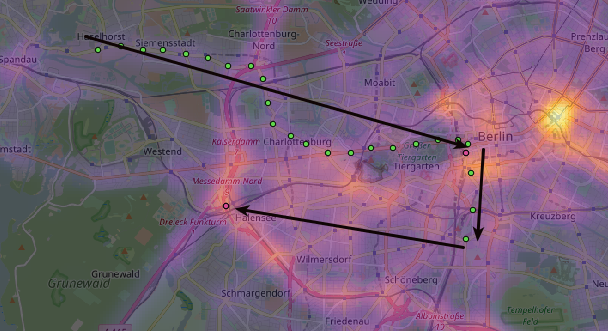
\includegraphics[width=0.6\textwidth]{images/reco_example_4a.png}\\
	\caption{ Visualization of distances, speed and mobility indexes for example from \autoref{fig:reco_ex_4b} with identified stop candidates }
	\label{fig:reco_ex_4a}
\end{figure} 
\begin{figure}[!ht]
	\centering
	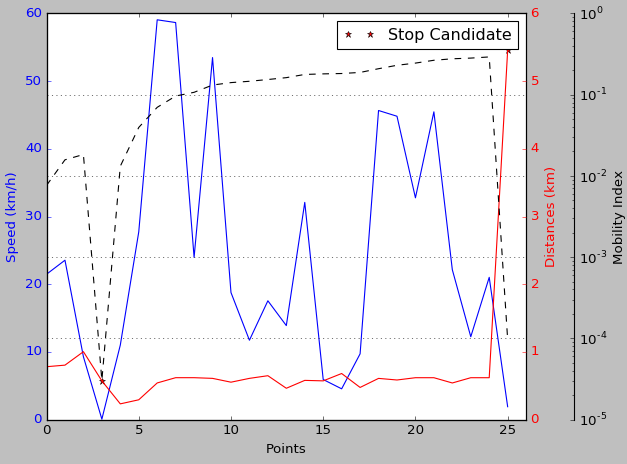
\includegraphics[width=0.6\textwidth]{images/reco_example_4b.png}\\
	\caption{ Movement example for one user in the period of 24h, with recorded locations due to the movement and annotated timestamps for detected stop candidates }
	\label{fig:reco_ex_4b}
\end{figure}
\end{appendices}

\end{document}
